\documentclass[12pt,a4paper]{article}

% --- Essential Packages ---
\usepackage[utf8]{inputenc}
\usepackage[T1]{fontenc}
\usepackage[margin=1in]{geometry}
\usepackage{setspace}
\onehalfspacing

\usepackage{graphicx}
\usepackage{amsmath,amssymb}
\usepackage{booktabs}
\usepackage{longtable}
\usepackage{tabularx}
\usepackage{caption}
\usepackage{subcaption}
\usepackage{float}
\usepackage{enumitem}
\usepackage{fancyhdr}
\usepackage{titlesec}
\usepackage{xcolor}
\usepackage[hyphens]{url}
\usepackage[colorlinks=true, linkcolor=blue!80!black, citecolor=green!60!black, urlcolor=blue!70!black]{hyperref}

% --- Code Listing Setup ---
\usepackage{listings}
\definecolor{javared}{rgb}{0.6,0,0}
\definecolor{javagreen}{rgb}{0.25,0.5,0.35}
\definecolor{javapurple}{rgb}{0.5,0,0.35}
\definecolor{javadocblue}{rgb}{0.25,0.35,0.75}
\definecolor{codebg}{rgb}{0.97,0.97,0.98}
\definecolor{framegray}{rgb}{0.85,0.85,0.88}

\lstset{
  language=Java,
  backgroundcolor=\color{codebg},
  basicstyle=\ttfamily\footnotesize,
  keywordstyle=\color{javapurple}\bfseries,
  stringstyle=\color{javared},
  commentstyle=\color{javagreen}\itshape,
  morecomment=[s][\color{javadocblue}]{/**}{*/},
  numbers=left,
  numberstyle=\tiny\color{gray},
  stepnumber=1,
  numbersep=8pt,
  showstringspaces=false,
  breaklines=true,
  frame=single,
  rulecolor=\color{framegray},
  tabsize=4,
  captionpos=b
}

% --- Header and Footer Configuration ---
\pagestyle{fancy}
\fancyhf{}
\fancyhead[L]{\small\nouppercase{\leftmark}}
\fancyhead[R]{\small Online Auction Management System}
\fancyfoot[C]{\thepage}
\renewcommand{\headrulewidth}{0.4pt}
\renewcommand{\footrulewidth}{0.4pt}

% --- Section Numbering & Styling ---
\titleformat{\section}{\Large\bfseries\color{blue!80!black}}{\thesection}{1em}{}
\titleformat{\subsection}{\large\bfseries\color{black!90}}{\thesubsection}{1em}{}
\titleformat{\subsubsection}{\normalsize\bfseries\color{black!80}}{\thesubsubsection}{1em}{}

\begin{document}

% ==============================================================================
% FRONT MATTER
% ==============================================================================
\begin{titlepage}
    \centering
    \vspace*{0.5cm}
    
    {\Huge \bfseries ONLINE AUCTION MANAGEMENT SYSTEM\par}
    \vspace{0.4cm}
    {\Large \textsc{BidNexus --- An Object-Oriented Desktop Auction Platform}\par}
    
    \vspace{1.2cm}
    \rule{0.8\textwidth}{1.5pt}\par
    \vspace{0.8cm}
    
    {\large \textbf{A Comprehensive Software Project Report Submitted in Partial Fulfillment of the Requirements for the Course:}\par}
    \vspace{0.3cm}
    {\Large \textbf{OBJECT-ORIENTED METHODOLOGIES (OOM)}\par}
    
    \vspace{1.2cm}
    
    \begin{minipage}{0.48\textwidth}
        \begin{flushleft} \large
            \textbf{Submitted By:}\\[0.2cm]
            \textbf{Student 1:} [Student Name 1] \\
            \textit{Roll No.:} [Roll Number 1]\\[0.15cm]
            \textbf{Student 2:} [Student Name 2] \\
            \textit{Roll No.:} [Roll Number 2]\\[0.15cm]
            \textbf{Student 3:} [Student Name 3] \\
            \textit{Roll No.:} [Roll Number 3]
        \end{flushleft}
    \end{minipage}
    \begin{minipage}{0.48\textwidth}
        \begin{flushright} \large
            \textbf{Under the Guidance of:}\\[0.2cm]
            \textbf{[Faculty Guide Name]}\\
            \textit{Designation:}\ [Assistant/Associate Professor]\\
            Department of Computer Science and Engineering
        \end{flushright}
    \end{minipage}
    
    \vfill
    
    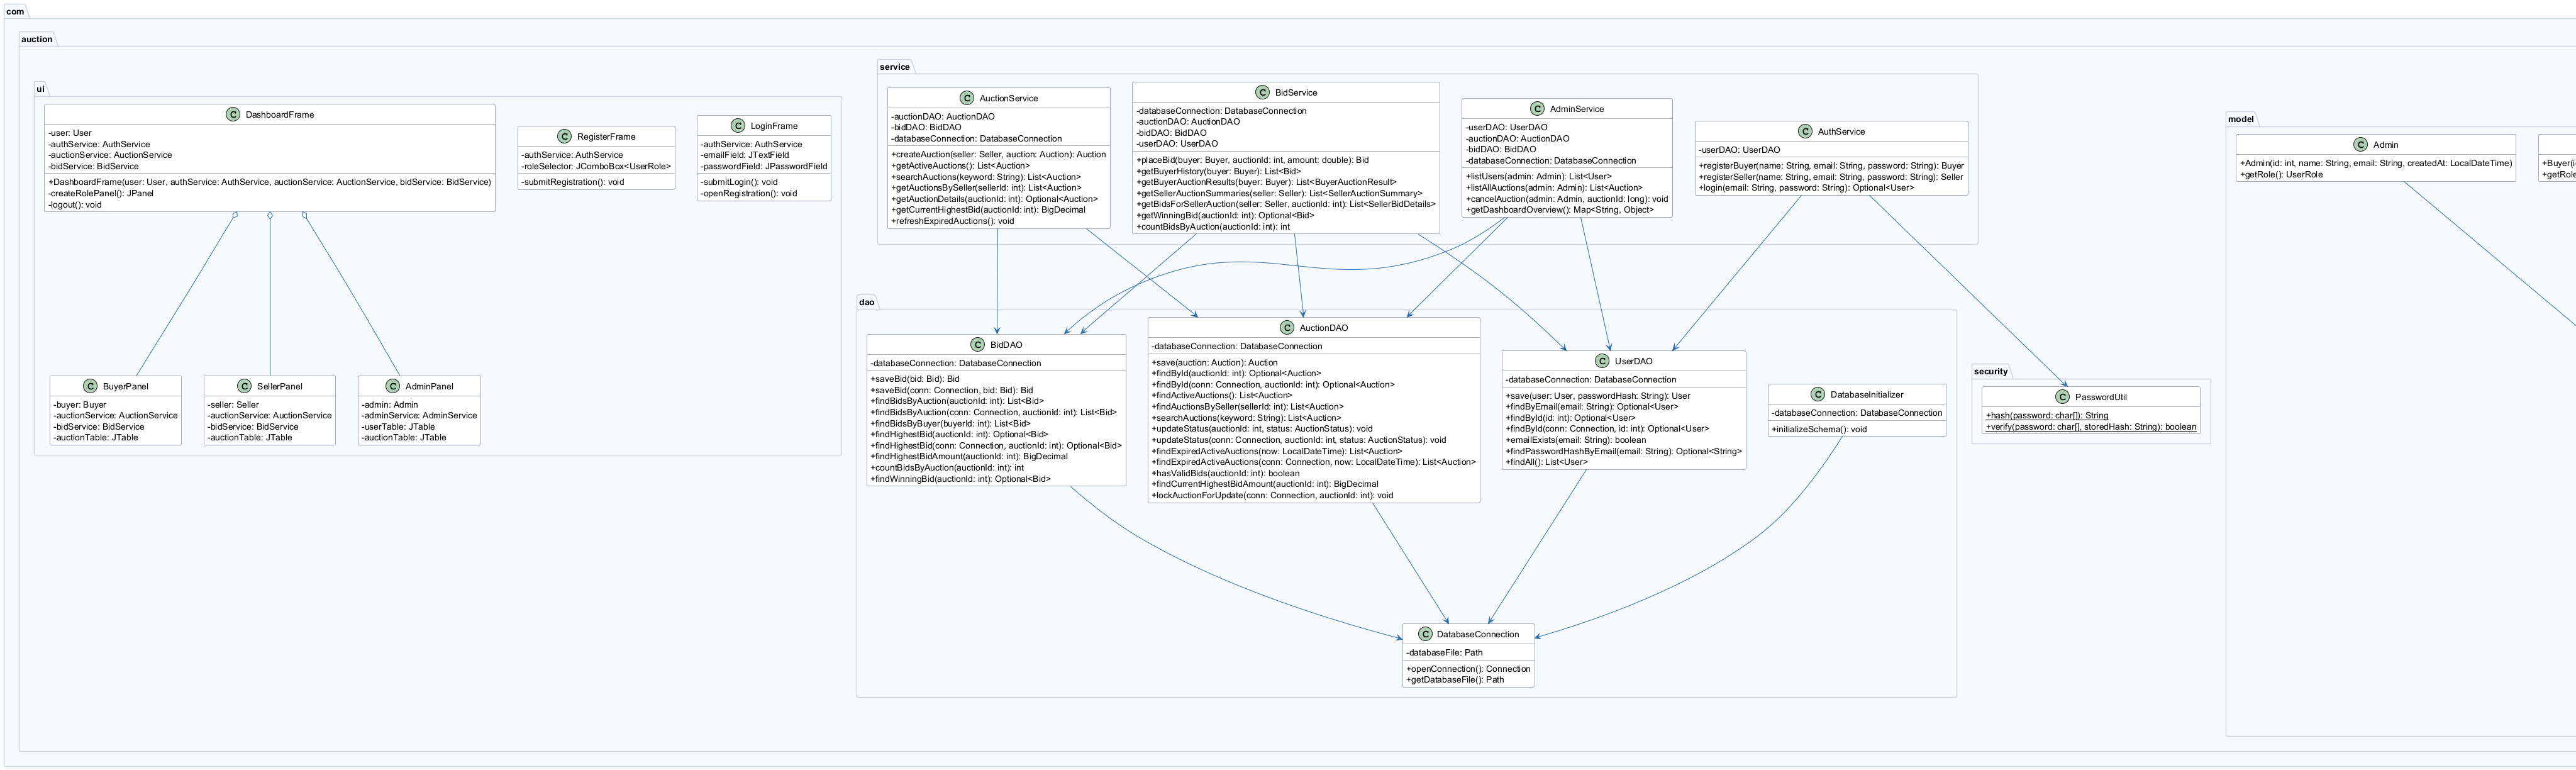
\includegraphics[width=0.22\textwidth]{figures/class_diagram.png}\\[0.3cm]
    {\small \textit{(Departmental Emblem / Project Illustration)}}\\[0.4cm]
    
    {\large \textbf{Department of Computer Science and Engineering}\par}
    {\large \textbf{[Institution / University Name]}\par}
    {\normalsize [City, State, Pin Code]}\par
    \vspace{0.4cm}
    {\large Academic Year: 2026--2027\par}
\end{titlepage}

\newpage
\pagenumbering{roman}
\setcounter{page}{2}

% --- Certificate ---
\section*{Certificate of Originality and Completion}
\addcontentsline{toc}{section}{Certificate of Originality and Completion}
\vspace{1cm}

This is to certify that the project entitled \textbf{``Online Auction Management System (BidNexus)''} is a bona fide record of academic project work carried out by:
\begin{center}
\begin{tabular}{llr}
\toprule
\textbf{Student Name} & \textbf{Roll Number} & \textbf{Branch / Semester} \\
\midrule
[Student Name 1] & [Roll Number 1] & B.Tech / B.E. CSE -- Sem VI \\
[Student Name 2] & [Roll Number 2] & B.Tech / B.E. CSE -- Sem VI \\
[Student Name 3] & [Roll Number 3] & B.Tech / B.E. CSE -- Sem VI \\
\bottomrule
\end{tabular}
\end{center}

\noindent in partial fulfillment of the academic requirements for the course \textbf{Object-Oriented Methodologies (OOM)} of the Bachelor of Technology / Engineering in Computer Science and Engineering during the academic session 2026--2027.

The work reported herein represents genuine system analysis, object-oriented design, architectural modeling, and software implementation executed under institutional supervision. It has not been submitted previously to any other institution for the award of any degree or diploma.

\vspace{3cm}

\noindent
\begin{minipage}[t]{0.32\textwidth}
\centering
\textbf{[Faculty Guide Name]}\\
\textit{Project Guide}\\
Dept. of CSE
\end{minipage}
\hfill
\begin{minipage}[t]{0.32\textwidth}
\centering
\textbf{[Head of Department]}\\
\textit{Head of Department}\\
Dept. of CSE
\end{minipage}
\hfill
\begin{minipage}[t]{0.32\textwidth}
\centering
\textbf{[External Examiner]}\\
\textit{External Examiner}\\
Institutional Seal
\end{minipage}

\newpage

% --- Declaration ---
\section*{Declaration by Authors}
\addcontentsline{toc}{section}{Declaration by Authors}
\vspace{1cm}

We hereby declare that the software project entitled \textbf{``Online Auction Management System (BidNexus)''} and this accompanying project report were independently researched, designed, coded, and verified by our project team under the esteemed guidance of \textbf{[Faculty Guide Name]}, Department of Computer Science and Engineering.

We confirm that:
\begin{enumerate}[label=(\alph*)]
    \item The object-oriented design models, UML diagrams, layered architectural implementations, and Java source code are authentic and developed specifically for this project.
    \item The underlying relational schema, transactional integrity controls, and concurrency mechanisms were designed and verified against the SQLite relational engine.
    \item All external ideas, published literature, reference frameworks, and toolkits (such as PlantUML, JUnit 5, and SQLite JDBC) have been duly recognized and cited in the bibliography.
    \item No portion of this project report has been plagiarized or submitted elsewhere for any academic credit or qualification.
\end{enumerate}

\vspace{2.5cm}

\noindent
\begin{minipage}[t]{0.32\textwidth}
\centering
\rule{4cm}{0.4pt}\\
\textbf{[Student Name 1]}\\
Roll No.: [Roll Number 1]
\end{minipage}
\hfill
\begin{minipage}[t]{0.32\textwidth}
\centering
\rule{4cm}{0.4pt}\\
\textbf{[Student Name 2]}\\
Roll No.: [Roll Number 2]
\end{minipage}
\hfill
\begin{minipage}[t]{0.32\textwidth}
\centering
\rule{4cm}{0.4pt}\\
\textbf{[Student Name 3]}\\
Roll No.: [Roll Number 3]
\end{minipage}

\vspace{1.5cm}
\noindent \textbf{Date:} November 18, 2026\\
\textbf{Place:} [City / Campus Name]

\newpage

% --- Acknowledgement ---
\section*{Acknowledgements}
\addcontentsline{toc}{section}{Acknowledgements}
\vspace{0.8cm}

We express our deepest sense of gratitude and respect to our revered project supervisor, \textbf{[Faculty Guide Name]}, for invaluable intellectual direction, rigorous reviews of our object-oriented designs, and constant encouragement throughout the development of the \textbf{Online Auction Management System (BidNexus)}.

We extend our sincere thanks to \textbf{[Head of Department]}, Head of the Department of Computer Science and Engineering, for providing excellent laboratory computing infrastructure and fostering an academic environment that champions software engineering rigor.

We are profoundly indebted to the faculty members and technical staff of the Department of Computer Science and Engineering for their direct and indirect support during our coursework in Object-Oriented Methodologies, Software Architecture, and Database Systems.

Finally, we express our heartfelt appreciation to our parents and friends whose unwavering encouragement and patience made the successful culmination of this software engineering endeavor possible.

\vspace{1.5cm}
\begin{flushright}
\textbf{Project Team}\\[0.1cm]
[Student Name 1] \quad [Student Name 2] \quad [Student Name 3]
\end{flushright}

\newpage

% --- Abstract ---
\section*{Abstract}
\addcontentsline{toc}{section}{Abstract}
\vspace{0.8cm}

The \textbf{Online Auction Management System (OAMS / BidNexus)} is an academic, production-grade desktop application engineered to demonstrate the practical application of \textbf{Object-Oriented Methodologies (OOM)}, software architecture patterns, and relational database integrity in real-time commerce. Traditional physical auctions and rudimentary electronic bidding systems frequently suffer from lack of transparency, architectural coupling, vulnerability to race conditions, and inadequate role-based access governance.

This project delivers a modular, layered desktop solution developed in modern \textbf{Java (JDK 17+)} using the \textbf{Java Swing GUI} toolkit and backed by an embedded \textbf{SQLite} database via JDBC. The system explicitly grounds its domain model upon the \textbf{Four Pillars of Object-Oriented Programming}:
\begin{itemize}[noitemsep]
    \item \textbf{Encapsulation:} Enforced via immutable domain entities (\texttt{User}, \texttt{Auction}, \texttt{Bid}) with private final fields, comprehensive constructor validation, and read-only exposure.
    \item \textbf{Inheritance:} Structured through an extensible hierarchical model where an abstract \texttt{User} base class is specialized into \texttt{Buyer}, \texttt{Seller}, and \texttt{Admin} subtypes.
    \item \textbf{Abstraction:} Implemented through decoupled service interfaces and abstract role contracts (\texttt{getRole()}), insulating GUI presentation from data persistence.
    \item \textbf{Polymorphism:} Realized through dynamic runtime dispatch, subtype substitution, and pattern matching switch expressions in role-tailored dashboard provisioning.
\end{itemize}

The system features robust business rule automation, including transactional bid placement with row-level locking to eliminate concurrent bid corruption, deterministic lazy auction expiration resolving listings into \texttt{SOLD} or \texttt{UNSOLD} states upon client access, and an integrated administrative monitoring console providing multi-field user search, auction status filtering, and policy-compliant auction cancellations. Complete automated test suites comprising 46 unit and integration test cases verify 100\% passing behavior across all domain constraints. This report provides an exhaustive technical analysis of system requirements, object-oriented analysis and design, UML specifications across eight standard modeling diagrams, architectural decisions, database schemas, and verification results.

\bigskip
\noindent \textbf{Keywords:} Object-Oriented Methodologies (OOM), Software Architecture, Encapsulation, Polymorphism, Unified Modeling Language (UML), Java Swing, SQLite JDBC, ACID Transactions, Auction Systems.

\newpage

% --- Table of Contents, Figures, Tables ---
\tableofcontents
\newpage
\listoffigures
\newpage
\listoftables
\newpage

\pagenumbering{arabic}
\setcounter{page}{1}

% ==============================================================================
% REPORT CHAPTERS
% ==============================================================================
\section{Introduction}
\label{sec:introduction}

\subsection{Project Background}
Auctions represent one of the oldest and most economically efficient mechanisms for price discovery and resource allocation in human commerce. In a conventional English auction, potential buyers assemble physically, submitting sequentially ascending bids for an asset until no participant is willing to surpass the prevailing highest bid. While effective in localized, physical settings, traditional auction models suffer from severe geographical barriers, high operational overhead, limited buyer participation, and substantial administrative latency in clearing transactions.

With the proliferation of modern computing infrastructure and networked software systems, digital auction platforms have fundamentally transformed commercial exchange. Platforms such as eBay demonstrated that automating auction mechanics enables global market liquidity, continuous trading, and transparent price formation. However, designing and implementing a dependable, real-time electronic auction system poses complex software engineering challenges. An online auction is inherently dynamic, stateful, and concurrent:
\begin{itemize}[noitemsep]
    \item Prices mutate rapidly under competitive bidding.
    \item Multi-user interactions must remain strictly synchronized to prevent race conditions.
    \item Temporal deadlines must be deterministically enforced to resolve listings into sold or unsold terminal states.
    \item Distinct actors---Buyers, Sellers, and System Administrators---possess conflicting responsibilities and access privileges that require airtight authorization boundaries.
\end{itemize}

The \textbf{Online Auction Management System (OAMS)}, academically designated as \textbf{BidNexus}, has been designed and implemented to provide a rigorous, production-grade demonstration of \textbf{Object-Oriented Methodologies (OOM)}. By applying core object-oriented principles, formalized Unified Modeling Language (UML) designs, layered architectural patterns, and relational persistence via SQLite and JDBC, the project bridges theoretical software engineering concepts with practical software development.

\subsection{Problem Statement}
Elementary implementations of auction software frequently suffer from architectural anti-patterns that render systems brittle, insecure, and unmaintainable. Common deficiencies observed in naive systems include:
\begin{enumerate}
    \item \textbf{Tight Coupling and Code Duplication:} Business logic, user interface components, and raw SQL queries are entangled within single monolithic classes, preventing modular testing or evolution.
    \item \textbf{Concurrency and Race Condition Vulnerabilities:} In concurrent multi-user environments, simultaneous bid submissions on the same auction item can lead to the ``lost update'' anomaly or permit a lower bid to overwrite a higher bid.
    \item \textbf{Unenforced Invariants and Primitive Obsession:} Relying on mutable public fields or raw primitive types (e.g., using unbounded integers or floating-point primitives without domain validation) leads to invalid domain states, such as negative bid amounts, auctions ending in the past, or sellers bidding on their own listings.
    \item \textbf{Ad-hoc Access Control and Security Vulnerabilities:} Passwords stored in plaintext or weak cryptographic hashes expose user accounts to compromise. A lack of role abstraction permits unauthorized users to execute administrative cancellations or perform privileged queries.
    \item \textbf{Unreliable Expiration Mechanics:} Systems that rely purely on client clocks or fragile background timer threads often fail to transition expired auctions accurately when background threads terminate unexpectedly.
\end{enumerate}

To address these vulnerabilities, this project establishes a disciplined, object-oriented framework that guarantees domain consistency, architectural separation of concerns, cryptographic security, and transactional database integrity.

\subsection{Project Objectives}
The primary academic and technical objectives of the Online Auction Management System are:
\begin{itemize}
    \item \textbf{Rigorous OOP Modeling:} Implement domain abstractions that directly embody the four pillars of Object-Oriented Programming: Encapsulation, Inheritance, Abstraction, and Polymorphism.
    \item \textbf{Layered Architectural Decoupling:} Maintain strict separation among Presentation (Java Swing GUI), Service/Business Logic, Security, and Data Access Objects (DAO).
    \item \textbf{ACID-Compliant Concurrency Management:} Implement row-level locking and transaction rollbacks in SQLite to guarantee serializable bid updates and eliminate race conditions.
    \item \textbf{Deterministic Lifecycle Automation:} Formulate a lazy-expiration mechanism that reliably evaluates auction termination criteria during user interactions without external scheduler dependencies.
    \item \textbf{Role-Based Access Governance:} Enforce role differentiation across Guests, Buyers, Sellers, and Administrators, providing dynamic UI generation and backend policy verification.
    \item \textbf{Complete Verification and Testability:} Validate all business rules, DAO operations, and service workflows through a 100\% passing automated JUnit 5 test suite.
\end{itemize}

\subsection{Scope of the Project}
The project delivers a fully functional, self-contained desktop system. The scope encompasses:
\begin{itemize}
    \item \textbf{Identity and Authentication Subsystem:} User registration and login for Buyers and Sellers; PBKDF2 with HMAC-SHA256 salted password hashing; role validation; session management.
    \item \textbf{Auction Management Subsystem:} Creation of auction listings with positive reserve prices, item categorization, and future expiration timestamps; multi-criteria search and retrieval.
    \item \textbf{Bidding and Settlement Subsystem:} Real-time competitive bidding with strict increment validation; automatic rejection of self-bidding; automatic winner determination upon auction expiration.
    \item \textbf{Administrative Subsystem:} System overview dashboard with real-time aggregated metrics; multi-attribute user search (ID, Name, Email, Role); comprehensive auction monitoring; policy-compliant listing cancellation.
    \item \textbf{Persistence Layer:} Fully normalized SQLite schema enforcing foreign key referential integrity via explicit \texttt{PRAGMA foreign\_keys = ON}.
\end{itemize}

\paragraph{Limitations and Future Enhancements (Deliberate Out-of-Scope Elements):}
In accordance with academic constraints, certain enterprise features are reserved for future work:
\begin{itemize}[noitemsep]
    \item Payment gateway integration (e.g., Stripe/PayPal) is represented as auction settlement status rather than active financial routing.
    \item Multi-tier network remoting (e.g., REST/WebSockets) is replaced by local multi-threaded client execution on a shared SQLite engine.
    \item Automated email/SMS dispatch upon winning an auction is tracked in-app via user dashboard history.
\end{itemize}

\subsection{Stakeholders and User Personas}
The system serves four distinct user classes:
\begin{enumerate}
    \item \textbf{Visitor / Guest:} Unauthenticated prospective users seeking to explore available auctions or create an account.
    \item \textbf{Buyer:} Authenticated users focused on querying active listings, evaluating pricing trends, placing bids, and tracking auction outcomes.
    \item \textbf{Seller:} Authenticated merchants who list items, configure starting prices and durations, and inspect bidding interest.
    \item \textbf{Administrator:} Trusted system overseers responsible for catalog health, user auditing, and moderating inappropriate or fraudulent listings.
\end{enumerate}

\subsection{Report Organization}
The remainder of this report is structured as follows:
\begin{itemize}[noitemsep]
    \item \textbf{Chapter \ref{sec:oop_methodology}:} Explores the Object-Oriented Methodology and details the realization of the Four Pillars in Java.
    \item \textbf{Chapter \ref{sec:requirements}:} Documents the Software Requirements Specification (SRS), functional/non-functional requirements, and use cases.
    \item \textbf{Chapter \ref{sec:uml_design}:} Presents all eight UML diagrams, explaining their architectural significance.
    \item \textbf{Chapter \ref{sec:architecture}:} Details the system architecture, design patterns, and package decomposition.
    \item \textbf{Chapter \ref{sec:technology_stack}:} Outlines the tools, libraries, and frameworks utilized.
    \item \textbf{Chapter \ref{sec:implementation}:} Walks through key implementation modules with real source code excerpts.
    \item \textbf{Chapter \ref{sec:database_design}:} Explains the SQLite relational schema, integrity constraints, and query strategies.
    \item \textbf{Chapter \ref{sec:testing}:} Reviews testing strategies, JUnit test cases, and verification metrics.
    \item \textbf{Chapter \ref{sec:screenshots}:} Provides visual walkthroughs of the graphical user interfaces.
    \item \textbf{Chapter \ref{sec:conclusion}:} Summarizes learnings, architectural contributions, and future scope.
\end{itemize}

\newpage
\section{Object-Oriented Methodology and Design Philosophy}
\label{sec:oop_methodology}

\subsection{Core Philosophy: Modeling the Real-World Domain}
Object-Oriented Methodologies (OOM) provide a paradigm for software engineering wherein systems are structured as cooperative collections of interacting, self-contained computational entities termed \textbf{objects}. Each object encapsulates both state (data attributes) and behavior (operations or methods) that directly correspond to real-world domain concepts. Rather than viewing software as a procedural sequence of instructions acting upon detached data structures, an object-oriented approach guarantees that data integrity, domain invariants, and operational policies are co-located within robust type abstractions \cite{bloch2018effective, gamma1994design}.

In the Online Auction Management System (BidNexus), the problem domain is inherently object-centric. An auction consists of discrete actors (Buyers, Sellers, Administrators) trading specific items (Auctions) through competitive offers (Bids). Applying OOM ensures that the system remains modular, resilient against concurrent state corruption, straightforward to test, and naturally extensible.

\subsection{The Four Pillars of Object-Oriented Programming}
The foundational architecture of BidNexus rests squarely upon the four pillars of Object-Oriented Programming: \textbf{Encapsulation}, \textbf{Inheritance}, \textbf{Abstraction}, and \textbf{Polymorphism}. The following sections provide an in-depth analysis of how each pillar is operationalized within genuine Java source code.

% --- Pillar 1: Encapsulation ---
\subsubsection{Pillar 1: Encapsulation and Invariant Preservation}
\textbf{Theoretical Definition:} Encapsulation is the mechanism that binds together data and the methods that manipulate that data, while shielding internal object representation from unauthorized external interference and misuse (information hiding). 

\paragraph{Implementation in BidNexus:}
In many vulnerable software systems, domain objects are treated as passive data holders (anemic domain models) with unrestricted public setters. This exposes internal state to inconsistent modifications (e.g., setting a negative bid or moving an auction end date into the past).

BidNexus strictly enforces encapsulation across all domain entities---\texttt{User}, \texttt{Auction}, and \texttt{Bid}---by adopting the \textbf{Immutable Domain Entity} pattern:
\begin{enumerate}
    \item \textbf{Private Final Fields:} All instance variables are declared \texttt{private final}. Once an object is constructed, its reference state cannot be reassigned.
    \item \textbf{Constructor-Level Invariant Enforcement:} Objects refuse construction unless all business invariants are validated at the constructor boundary.
    \item \textbf{Absence of Public Mutators:} The classes expose no public setters. Mutation of business state (such as updating an auction status in the database) is handled via explicit transactional service methods rather than in-memory mutation.
\end{enumerate}

Listing \ref{lst:user_encapsulation} highlights encapsulation within the \texttt{User} class.

\begin{lstlisting}[caption={Encapsulation and Invariant Checking in \texttt{User.java}}, label={lst:user_encapsulation}]
public abstract class User {
    private static final Pattern EMAIL_PATTERN = 
        Pattern.compile("^[^\\s@]+@[^\\s@]+\\.[^\\s@]+$");

    // Strictly encapsulated private final attributes
    private final int id;
    private final String name;
    private final String email;
    private final LocalDateTime createdAt;

    protected User(int id, String name, String email, LocalDateTime createdAt) {
        if (id < 0) {
            throw new IllegalArgumentException("User id cannot be negative");
        }
        String normalizedName = Objects.requireNonNull(name, "name").trim();
        if (normalizedName.isEmpty() || normalizedName.length() > 100) {
            throw new IllegalArgumentException("Name must contain 1 to 100 characters");
        }
        String normalizedEmail = normalizeEmail(email);
        if (normalizedEmail.length() > 254 || !EMAIL_PATTERN.matcher(normalizedEmail).matches()) {
            throw new IllegalArgumentException("A valid email address is required");
        }

        this.id = id;
        this.name = normalizedName;
        this.email = normalizedEmail;
        this.createdAt = createdAt;
    }

    public static String normalizeEmail(String email) {
        return Objects.requireNonNull(email, "email").trim().toLowerCase(Locale.ROOT);
    }

    // Read-only accessors shield internal state
    public int getId() { return id; }
    public String getName() { return name; }
    public String getEmail() { return email; }
    public LocalDateTime getCreatedAt() { return createdAt; }
    public abstract UserRole getRole();
}
\end{lstlisting}

Similarly, the \texttt{Auction} class encapsulates time-based lifecycle evaluation through its \texttt{isExpired()} method (Listing \ref{lst:auction_encapsulation}), eliminating the risk of external components calculating expiration inconsistently.

\begin{lstlisting}[caption={Encapsulated Domain Logic in \texttt{Auction.java}}, label={lst:auction_encapsulation}]
public final class Auction {
    private final int id;
    private final int sellerId;
    private final String productName;
    private final BigDecimal startingPrice;
    private final LocalDateTime endTime;
    private final AuctionStatus status;
    // ... Additional fields omitted for brevity ...

    public boolean isExpired() {
        return isExpired(LocalDateTime.now());
    }

    public boolean isExpired(LocalDateTime now) {
        return !Objects.requireNonNull(now, "now").isBefore(endTime);
    }
}
\end{lstlisting}

% --- Pillar 2: Inheritance ---
\subsubsection{Pillar 2: Inheritance and Generalization Hierarchies}
\textbf{Theoretical Definition:} Inheritance is the object-oriented mechanism by which a specialized derived class (subclass) inherits attributes and behaviors from a generalized base class (superclass), promoting code reuse and establishing an ``IS-A'' taxonomic relationship.

\paragraph{Implementation in BidNexus:}
In BidNexus, users of the platform share foundational identity attributes: each possesses a unique database identifier, a full name, a validated email address, and an account creation timestamp. However, each user acts in a distinct operational capacity.

Rather than duplicating identity fields across separate disparate classes or employing a single monolithic user class littered with nullable role fields, BidNexus implements an inheritance hierarchy:
\begin{itemize}
    \item \texttt{User} acts as the abstract superclass providing common identity management and validation logic.
    \item \texttt{Buyer}, \texttt{Seller}, and \texttt{Admin} extend \texttt{User} as concrete subclasses.
\end{itemize}

Listing \ref{lst:buyer_inheritance} demonstrates how \texttt{Buyer} extends \texttt{User}, invoking the base constructor via \texttt{super(...)} to reuse identity validation and establishing subclass specialization.

\begin{lstlisting}[caption={Subclass Specialization via Inheritance in \texttt{Buyer.java}}, label={lst:buyer_inheritance}]
public final class Buyer extends User {

    public Buyer(String name, String email) {
        this(0, name, email, LocalDateTime.now());
    }

    public Buyer(int id, String name, String email, LocalDateTime createdAt) {
        super(id, name, email, createdAt); // Invokes base validation
    }

    @Override
    public UserRole getRole() {
        return UserRole.BUYER; // Subclass-specific specialization
    }
}
\end{lstlisting}

This taxonomy ensures that common user behavior is maintained in exactly one place (the superclass), adhering strictly to the Don't Repeat Yourself (DRY) principle.

% --- Pillar 3: Abstraction ---
\subsubsection{Pillar 3: Abstraction and Interface Contracts}
\textbf{Theoretical Definition:} Abstraction is the intentional suppression of complex, irrelevant implementation details in favor of essential high-level behavioral contracts. It enables developers to interact with components via stable interfaces without concern for underlying mechanics.

\paragraph{Implementation in BidNexus:}
Abstraction operates at multiple architectural tiers within BidNexus:
\begin{enumerate}
    \item \textbf{Model-Level Behavioral Abstraction:} The \texttt{User} superclass declares the abstract method:
    \begin{center}
    \texttt{public abstract UserRole getRole();}
    \end{center}
    The base class does not define how a role is determined; instead, it establishes an abstract contract that all concrete user subtypes must fulfill.
    \item \textbf{Layered Service Abstraction:} The Presentation Layer (Swing GUI) never communicates directly with SQL queries, SQLite JDBC drivers, or database connections. Instead, it interacts with high-level service abstractions:
    \begin{itemize}
        \item \texttt{AuthService}: Abstracts password hashing, salt generation, and credential verification into simple methods like \texttt{login(email, password)}.
        \item \texttt{BidService}: Abstracts ACID transaction boundaries, row-level locks, and price comparison rules into a unified \texttt{placeBid(buyer, auctionId, amount)} call.
        \item \texttt{AdminService}: Abstracts multi-table joins and aggregation queries into \texttt{getDashboardOverview()} and \texttt{cancelAuction(admin, auctionId)}.
    \end{itemize}
\end{enumerate}

By hiding the complexities of database transaction handling and cryptographic algorithms behind clean service interfaces, the system achieves loose coupling and high maintainability.

% --- Pillar 4: Polymorphism ---
\subsubsection{Pillar 4: Polymorphism and Dynamic Method Dispatch}
\textbf{Theoretical Definition:} Polymorphism (``many forms'') allows entities of different specific types to be handled through a common generic interface, with the specific execution behavior dynamically resolved at runtime (dynamic binding).

\paragraph{Implementation in BidNexus:}
Polymorphism is extensively utilized across BidNexus in both the domain layer and presentation workflows:
\begin{enumerate}
    \item \textbf{Subtype Polymorphism via Abstract Method Dispatch:} When the system retrieves a collection of registered users from the database, the Data Access Layer returns a polymorphic \texttt{List<User>}. Each element in the list is an instance of \texttt{Buyer}, \texttt{Seller}, or \texttt{Admin}. Invoking \texttt{user.getRole()} triggers dynamic method dispatch, executing the subclass-specific override at runtime without requiring brittle conditional type checks.
    \item \textbf{Polymorphic UI Provisioning (Pattern Matching):} When a user successfully authenticates, the system launches \texttt{DashboardFrame(User user, ...)}. The dashboard dynamically provisions role-tailored workspaces based on the runtime type of the user, leveraging modern Java pattern matching and switch expressions as illustrated in Listing \ref{lst:dashboard_polymorphism}.
\end{enumerate}

\begin{lstlisting}[caption={Polymorphic Dashboard Page Dispatch in \texttt{DashboardFrame.java}}, label={lst:dashboard_polymorphism}]
private JPanel createDashboardPage(String page) {
    // Dynamic dispatch depending on the polymorphic role of the user
    return switch (user.getRole()) {
        case BUYER  -> createBuyerPage(page);
        case SELLER -> createSellerPage(page);
        case ADMIN  -> createAdminPage(page);
    };
}

private JPanel createBuyerPage(String page) {
    // Java 17 pattern matching for instanceof
    if (user instanceof Buyer buyer) {
        return switch (page) {
            case "Overview"        -> new BuyerPanel(buyer, auctionService, bidService);
            case "Browse auctions" -> new BuyerPanel(buyer, auctionService, bidService);
            case "My bids"         -> buildBuyerTablePage("My Bids", ...);
            case "Auction history" -> buildBuyerTablePage("Auction Results", ...);
            default -> throw new IllegalArgumentException("Unknown page: " + page);
        };
    }
    throw new IllegalStateException("BUYER role does not match account type");
}
\end{lstlisting}

\subsection{Comparative Analysis: OOP Concepts vs. Project Implementation}
Table \ref{tab:oop_comparison} synthesizes how theoretical OOP principles are concretely mapped into the BidNexus codebase, demonstrating alignment between academic theory and practical software construction.

\begin{table}[H]
\centering
\small
\caption{Systematic Mapping of OOP Concepts to BidNexus Source Implementation}
\label{tab:oop_comparison}
\begin{tabularx}{\textwidth}{p{2.8cm}p{4cm}p{4.2cm}X}
\toprule
\textbf{OOP Concept} & \textbf{Theoretical Definition} & \textbf{BidNexus Implementation} & \textbf{Architectural Benefit} \\
\midrule
\textbf{Encapsulation} & Bundling state and methods; hiding internal representations. & \texttt{User}, \texttt{Auction}, \texttt{Bid} classes use \texttt{private final} fields and constructor validation. & Prevents illegal state; guarantees immutable domain models. \\
\addlinespace
\textbf{Inheritance} & Deriving specialized classes from a generalized base class. & \texttt{Buyer}, \texttt{Seller}, \texttt{Admin} extend \texttt{abstract class User}. & Eliminates redundant code; centralizes identity validation. \\
\addlinespace
\textbf{Abstraction} & Exposing essential behavior while concealing implementation details. & Abstract method \texttt{getRole()}; Service interfaces (\texttt{BidService}, \texttt{AuthService}). & Insulates GUI from raw SQL, transactions, and cryptography. \\
\addlinespace
\textbf{Polymorphism} & Treating diverse subtypes uniformly through common interfaces. & Runtime dispatch of \texttt{user.getRole()}; pattern matching in \texttt{DashboardFrame}. & Enables dynamic UI rendering and role-based policy enforcement. \\
\addlinespace
\textbf{Cohesion} & Degree to which elements inside a module belong together. & Layered separation: Model (state), DAO (persistence), Service (rules). & High cohesion ensures single-responsibility compliance. \\
\addlinespace
\textbf{Loose Coupling} & Minimizing interdependencies between components. & Dependency injection of DAOs and connections into service layers. & Facilitates isolated unit testing using in-memory databases. \\
\bottomrule
\end{tabularx}
\end{table}

\newpage
\section{System Requirements and Specifications}
\label{sec:requirements}

\subsection{Software Requirements Specification (SRS) Overview}
The Software Requirements Specification (SRS) establishes a formal baseline describing the operational capabilities, environmental constraints, user interactions, and performance characteristics of the Online Auction Management System (BidNexus). In object-oriented systems engineering, rigorous requirement modeling is essential to identify candidate entity types, delineate system boundaries, and define class responsibilities before committing to architectural design.

\subsection{User Personas and Actor Delineation}
The system defines four principal actors, each associated with specific roles, capabilities, and system expectations:
\begin{enumerate}
    \item \textbf{Guest / Visitor (Unauthenticated Actor):} Any user who accesses the application prior to authentication. Guests are permitted to inspect basic application metadata and proceed to either User Registration or Login.
    \item \textbf{Buyer (Registered Actor):} An authenticated customer whose primary objective is commercial acquisition. Buyers browse active auction listings, execute keyword searches, submit competitive financial bids, inspect personal bidding histories, and monitor won or lost auction outcomes.
    \item \textbf{Seller (Registered Actor):} An authenticated merchant whose objective is item liquidation. Sellers create structured auction listings specifying product details, categories, starting reserve prices, and durations. Sellers monitor bidding activity and review closing outcomes.
    \item \textbf{System Administrator (Privileged Actor):} A system operator entrusted with catalog moderation, governance, and audit operations. Administrators view aggregated platform metrics, search and filter all registered users and auctions, inspect detailed audit logs, and cancel compromised or fraudulent active listings.
\end{enumerate}

\subsection{Functional Requirements}
The functional capabilities of BidNexus are organized into five primary functional domains:

\paragraph{Domain 1: Identity, Authentication, and Session Management}
\begin{itemize}
    \item \textbf{FR-1 (Registration):} The system shall allow visitors to register an account by providing their full name, a valid RFC-5322 compliant email address, a password, and a designated primary role (\texttt{BUYER} or \texttt{SELLER}). Duplicate email registrations must be rejected.
    \item \textbf{FR-2 (Password Security):} The system shall hash all passwords using PBKDF2WithHmacSHA256 with a unique cryptographic salt and high iteration count prior to persistence. Plaintext passwords must never be stored, logged, or exposed in the UI.
    \item \textbf{FR-3 (Authentication):} The system shall authenticate users against their registered email and password. Upon successful validation, the system shall establish an active user session and dynamically launch the corresponding role dashboard.
    \item \textbf{FR-4 (Session Clearance / Logout):} The system shall provide an explicit Logout action that invalidates the current session, disposes of open workspace windows, and returns the user to the initial Login interface.
\end{itemize}

\paragraph{Domain 2: Auction Management and Catalog Browsing}
\begin{itemize}
    \item \textbf{FR-5 (Auction Listing Creation):} The system shall enable Sellers to list items by specifying product name, optional category, optional description, a starting price strictly greater than zero, and an expiration timestamp occurring strictly in the future. Initial listing status must be set to \texttt{ACTIVE}.
    \item \textbf{FR-6 (Catalog Exploration and Search):} The system shall allow Buyers to view all \texttt{ACTIVE} auctions. Users can perform case-insensitive substring searches across product names and categories.
    \item \textbf{FR-7 (Auction Details Inspection):} The system shall provide detailed views for any selected listing, showing product information, seller identification, starting price, prevailing highest bid, and remaining bidding duration.
\end{itemize}

\paragraph{Domain 3: Bidding Operations and Concurrency Protection}
\begin{itemize}
    \item \textbf{FR-8 (Competitive Bid Submission):} The system shall allow authenticated Buyers to place bids on active listings. A submitted bid must be strictly greater than the current highest bid (or strictly greater than the starting price if no previous bids exist).
    \item \textbf{FR-9 (Self-Bidding Restriction):} The system shall reject any bid submission where the buyer's user ID matches the seller ID of the target auction (anti-shill bidding policy).
    \item \textbf{FR-10 (Transactional Concurrency Control):} The system shall execute bid placement within an ACID transaction utilizing row-level update locking in SQLite, ensuring that simultaneous bids are serialized and preventing lost update race conditions.
\end{itemize}

\paragraph{Domain 4: Automated Lifecycle and Settlement Mechanics}
\begin{itemize}
    \item \textbf{FR-11 (Lazy Expiration Resolution):} The system shall evaluate the timestamp of active auctions upon any catalog query or bid submission. If the current time exceeds the expiration time:
    \begin{itemize}
        \item If at least one valid bid exists, the auction status transitions to \texttt{SOLD}, and the highest bidder is designated as the winning buyer.
        \item If zero bids exist, the auction status transitions to \texttt{UNSOLD}.
    \end{itemize}
    \item \textbf{FR-12 (Participant Activity Tracking):} The system shall provide Buyers with a dedicated ``My Bids'' view and an ``Auction Results'' view displaying won, lost, and active participation records. Sellers shall have access to summarized listing activity and itemized bid histories.
\end{itemize}

\paragraph{Domain 5: Administrative Governance and Moderation}
\begin{itemize}
    \item \textbf{FR-13 (Dashboard Overview Metrics):} The Admin Panel shall compute and display live statistical summary cards directly from the database: Total Users, Total Buyers, Total Sellers, Total Admins, Total Auctions, Active Auctions, Sold Auctions, Unsold Auctions, and Cancelled Auctions.
    \item \textbf{FR-14 (User Management and Multi-Criteria Filtering):} Administrators can view all users in a tabular format, search by ID, Name, or Email, and filter by role (\texttt{BUYER} or \texttt{SELLER}). Selecting a user allows opening a detailed profile modal.
    \item \textbf{FR-15 (Auction Monitoring and Moderation):} Administrators can monitor all platform auctions across all lifecycle states, search by product name, seller, or ID, filter by status, and view complete bid logs in an Auction Details modal.
    \item \textbf{FR-16 (Listing Cancellation):} Administrators can cancel an active auction. The system verifies that the listing is currently \texttt{ACTIVE}, prompts for confirmation, updates the status to \texttt{CANCELLED}, and updates dashboard metrics. Non-active auctions cannot be cancelled.
\end{itemize}

\subsection{Non-Functional Requirements (NFRs)}
Non-functional requirements specify qualitative attributes of the software, summarized in Table \ref{tab:nfr_summary}.

\begin{table}[H]
\centering
\small
\caption{Non-Functional Requirements Specification}
\label{tab:nfr_summary}
\begin{tabularx}{\textwidth}{p{3.2cm}p{4cm}X}
\toprule
\textbf{Quality Attribute} & \textbf{Requirement Metric} & \textbf{Architectural Realization} \\
\midrule
\textbf{Performance} & Query execution and UI table rendering $< 100$\,ms for catalogs up to $10^4$ records. & Indexed columns (\texttt{product\_name}, \texttt{status}, \texttt{seller\_id}); background \texttt{SwingWorker} threads for non-blocking UI. \\
\addlinespace
\textbf{Data Integrity} & 100\% ACID compliance; zero orphaned records or negative prices. & SQLite foreign keys enabled via \texttt{PRAGMA foreign\_keys = ON}; database CHECK constraints; JDBC transaction boundaries. \\
\addlinespace
\textbf{Security} & Complete protection of credentials; zero SQL injection vulnerability. & PBKDF2 salted password hashing; 100\% parameterized SQL via \texttt{PreparedStatement}; role verification in service layer. \\
\addlinespace
\textbf{Fault Tolerance} & Graceful recovery from database locking or bad input; no silent blanks. & Robust exception propagation; informative user dialogs; transaction rollbacks in \texttt{catch} blocks. \\
\addlinespace
\textbf{Usability} & Modern, consistent desktop interface; responsive layout. & Unified \texttt{UiStyle} palette; clear typography; tabular views with scroll panes; confirmation dialogs on destructive actions. \\
\addlinespace
\textbf{Maintainability} & Modular decoupling; strict separation of concerns. & Strict layered architecture (GUI $\rightarrow$ Service $\rightarrow$ DAO $\rightarrow$ DB); high test coverage via JUnit 5. \\
\bottomrule
\end{tabularx}
\end{table}

\subsection{Detailed Use Case Specifications}
To formalize user-system interactions, Tables \ref{tab:uc_bid} and \ref{tab:uc_cancel} present detailed specifications for two core scenarios: placing a bid and cancelling an auction.

\begin{table}[H]
\centering
\small
\caption{Use Case Specification: UC-05 Place Competitive Bid}
\label{tab:uc_bid}
\begin{tabularx}{\textwidth}{p{3.5cm}X}
\toprule
\textbf{Field} & \textbf{Specification} \\
\midrule
\textbf{Use Case ID} & UC-05 \\
\textbf{Use Case Name} & Place Competitive Bid \\
\textbf{Primary Actor} & Buyer (Authenticated) \\
\textbf{Preconditions} & 1. Buyer is successfully authenticated.\\
                       & 2. Target auction listing has \texttt{ACTIVE} status and has not expired.\\
                       & 3. Buyer does not own the target auction listing. \\
\textbf{Main Success Scenario} & 1. Buyer browses or searches active auctions on the Buyer Dashboard.\\
                               & 2. Buyer selects an auction item and clicks ``Place Bid''.\\
                               & 3. Buyer inputs a bid amount in the bid dialog and confirms submission.\\
                               & 4. System initiates an ACID database transaction and acquires a row lock.\\
                               & 5. System verifies buyer identity, auction status, and checks that current time $<$ end time.\\
                               & 6. System validates that the bid amount exceeds the current highest bid (or starting price).\\
                               & 7. System inserts the new bid into the \texttt{bids} table.\\
                               & 8. System commits the transaction and updates UI bidding tables.\\
                               & 9. System displays a success confirmation message to the Buyer.\\
\textbf{Extensions / Alternative Flows} & \textbf{5a. Auction expired during submission:}\\
                                        & \quad 5a1. System lazily resolves auction to \texttt{SOLD} or \texttt{UNSOLD}.\\
                                        & \quad 5a2. System commits status change, rolls back bid, and notifies Buyer.\\
                                        & \textbf{6a. Bid amount is insufficient:}\\
                                        & \quad 6a1. System rolls back transaction.\\
                                        & \quad 6a2. System displays error message stating the required minimum amount.\\
\textbf{Postconditions} & A valid bid record is persisted in SQLite; the auction's highest bid is updated. \\
\bottomrule
\end{tabularx}
\end{table}

\begin{table}[H]
\centering
\small
\caption{Use Case Specification: UC-12 Cancel Active Auction Listing}
\label{tab:uc_cancel}
\begin{tabularx}{\textwidth}{p{3.5cm}X}
\toprule
\textbf{Field} & \textbf{Specification} \\
\midrule
\textbf{Use Case ID} & UC-12 \\
\textbf{Use Case Name} & Cancel Active Auction Listing \\
\textbf{Primary Actor} & System Administrator (Authenticated) \\
\textbf{Preconditions} & 1. User is authenticated with \texttt{ADMIN} role.\\
                       & 2. Target auction exists in SQLite database with \texttt{ACTIVE} status. \\
\textbf{Main Success Scenario} & 1. Administrator navigates to the ``Auction Monitoring'' tab in Admin Panel.\\
                               & 2. Administrator selects an active auction row from the table.\\
                               & 3. Administrator clicks the ``Cancel Auction'' button.\\
                               & 4. System displays a modal confirmation dialog requesting verification.\\
                               & 5. Administrator confirms the cancellation action.\\
                               & 6. System invokes \texttt{AdminService.cancelAuction(admin, auctionId)}.\\
                               & 7. System verifies admin privileges and checks that the auction status is \texttt{ACTIVE}.\\
                               & 8. System executes an \texttt{UPDATE} statement setting status to \texttt{CANCELLED}.\\
                               & 9. System refreshes the auction table and updates dashboard statistics cards.\\
                               & 10. System displays a success confirmation dialog. \\
\textbf{Extensions / Alternative Flows} & \textbf{7a. Auction status is not ACTIVE (already SOLD, UNSOLD, or CANCELLED):}\\
                                        & \quad 7a1. System rejects the cancellation request.\\
                                        & \quad 7a2. System displays an error stating non-active listings cannot be cancelled.\\
\textbf{Postconditions} & The target auction's status is permanently set to \texttt{CANCELLED} in the database. \\
\bottomrule
\end{tabularx}
\end{table}

\newpage
\section{Object-Oriented Modeling and UML Design}
\label{sec:uml_design}

\subsection{Overview of UML Modeling in System Engineering}
The Unified Modeling Language (UML) is the industry-standard visual modeling language used to specify, visualize, construct, and document the artifacts of software-intensive systems \cite{fowler2003uml}. In an Object-Oriented Methodologies curriculum, UML serves as the conceptual blueprint bridging high-level functional requirements and concrete object-oriented source code.

This chapter presents an exhaustive architectural analysis of the Online Auction Management System (BidNexus) across eight standard UML diagram types: Use Case, Class, Sequence (five detailed scenarios), Activity, State Machine, Component, Deployment, and Entity-Relationship. All diagrams were modeled formally in PlantUML and rendered to high-resolution vector/raster graphics directly reflecting the underlying Java implementation.

% ==============================================================================
% 1. USE CASE DIAGRAM
% ==============================================================================
\subsection{Use Case Diagram}
\label{subsec:uml_use_case}

\subsubsection{Diagram Visualization}
Figure \ref{fig:use_case} depicts the high-level functional capabilities exposed to the system's human actors.

\begin{figure}[H]
    \centering
    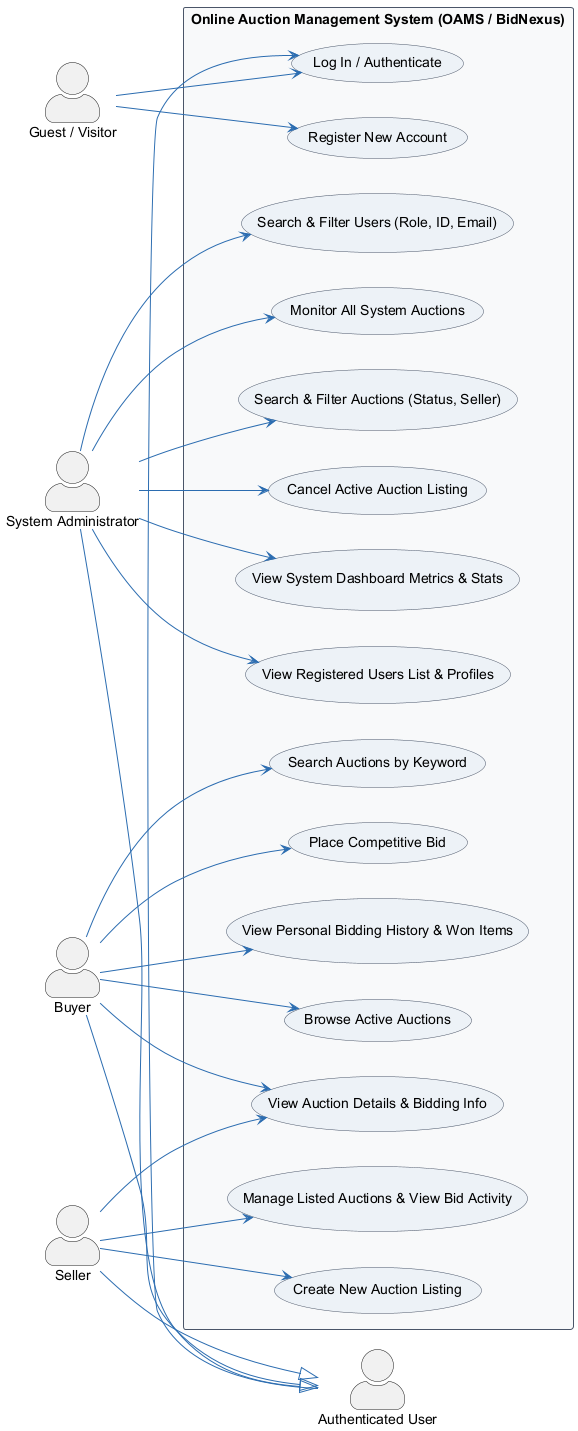
\includegraphics[width=0.95\textwidth]{figures/use_case_diagram.png}
    \caption{UML Use Case Diagram for Online Auction Management System}
    \label{fig:use_case}
\end{figure}

\subsubsection{Structural and Behavioral Analysis}
The Use Case diagram delineates the system boundary of BidNexus and models actor interactions:
\begin{itemize}
    \item \textbf{Actor Hierarchy and Generalization:} An unauthenticated actor begins as a \textit{Guest / Visitor}, restricted to registering an account or initiating login. Upon successful authentication, the actor generalizes into an \textit{Authenticated User}. \textit{Buyer}, \textit{Seller}, and \textit{System Administrator} inherit this authenticated base status while branching into specialized roles.
    \item \textbf{Buyer Domain Use Cases:} Buyers interact with use cases governing catalog exploration and purchase: \textit{Browse Active Auctions}, \textit{Search Auctions by Keyword}, \textit{View Auction Details}, \textit{Place Competitive Bid}, and \textit{View Personal Bidding History \& Won Items}.
    \item \textbf{Seller Domain Use Cases:} Sellers interact with inventory liquidation features: \textit{Create New Auction Listing}, \textit{Manage Listed Auctions}, and \textit{Inspect Received Bids}.
    \item \textbf{Administrator Domain Use Cases:} Privileged operators interact with system governance functions: \textit{View Registered Users List}, \textit{Search \& Filter Users}, \textit{Monitor All System Auctions}, \textit{Filter Auctions by Status}, \textit{Cancel Active Listing}, and \textit{View System Dashboard Metrics}.
\end{itemize}

% ==============================================================================
% 2. CLASS DIAGRAM
% ==============================================================================
\subsection{Class Diagram (Structural Architecture)}
\label{subsec:uml_class}

\subsubsection{Diagram Visualization}
Figure \ref{fig:class_diagram} illustrates the static structural design of BidNexus, detailing classes, attributes, operations, visibility modifiers, and inter-class relationships.

\begin{figure}[H]
    \centering
    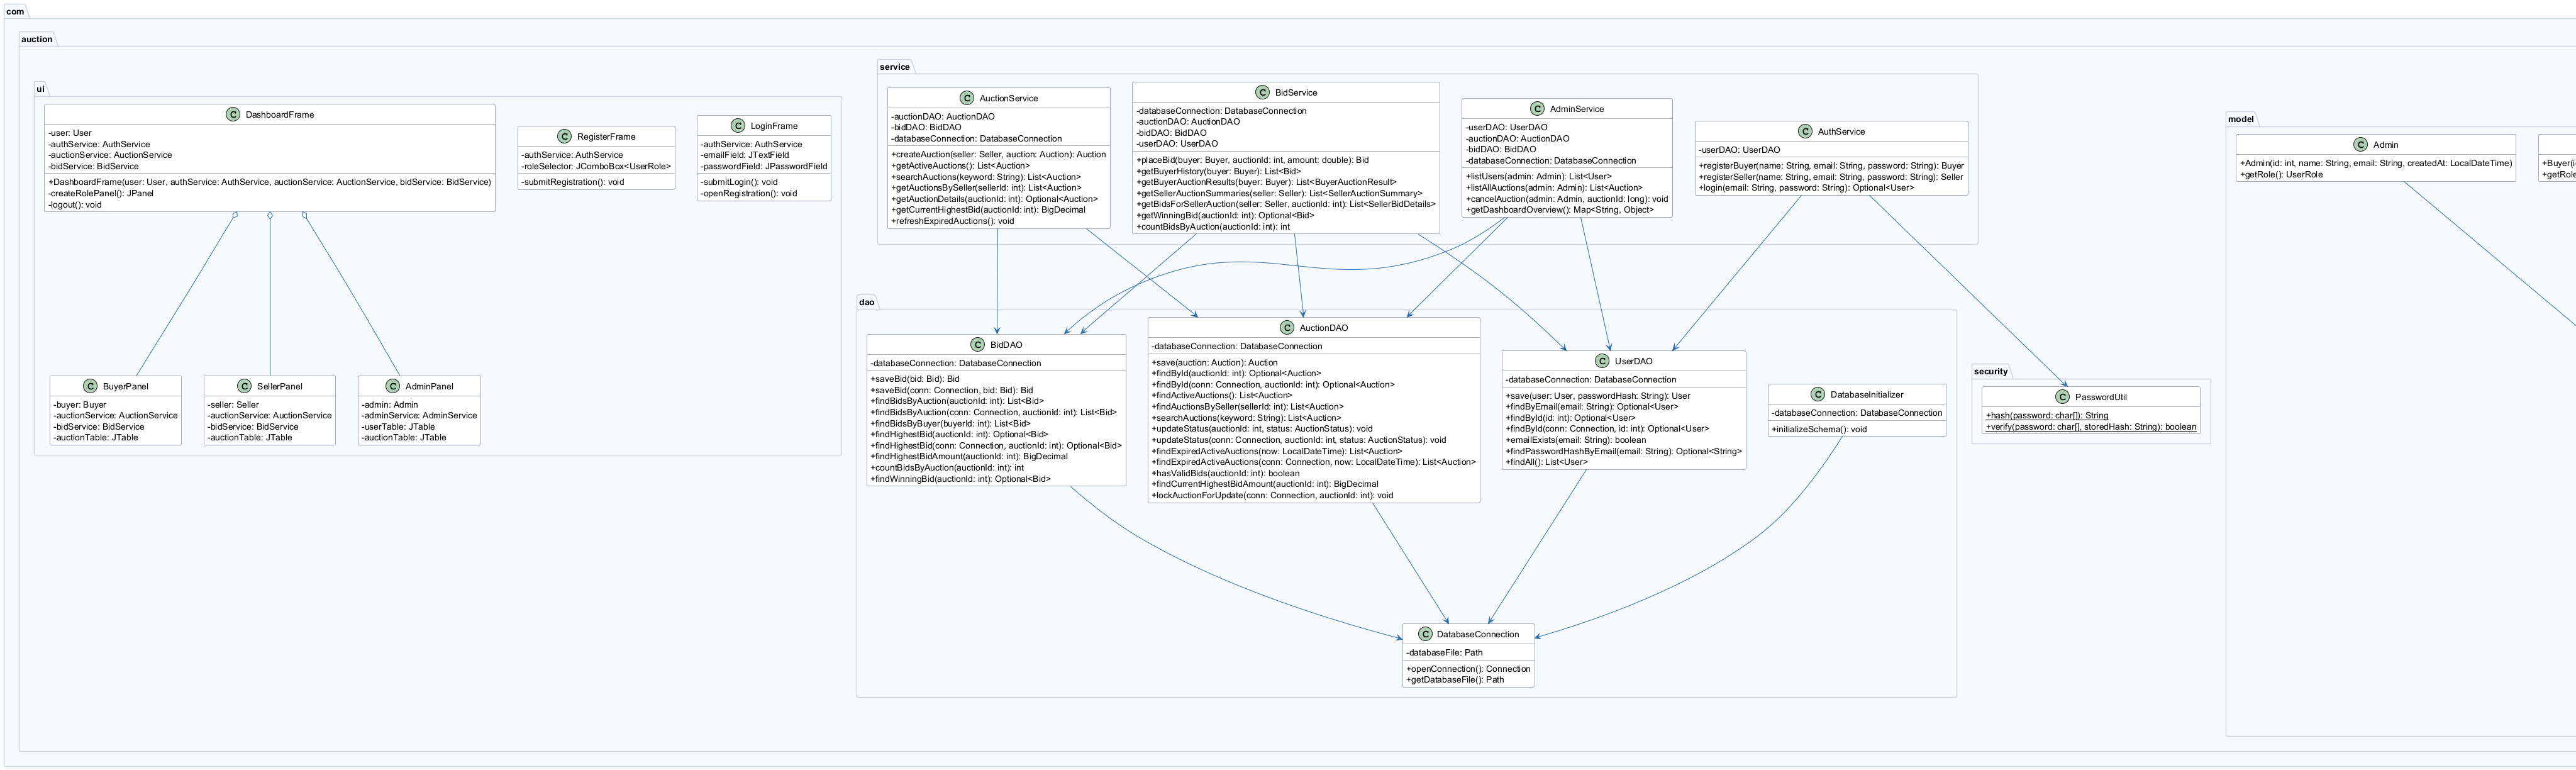
\includegraphics[width=\textwidth]{figures/class_diagram.png}
    \caption{UML Class Diagram Depicting Model, Service, DAO, and GUI Packages}
    \label{fig:class_diagram}
\end{figure}

\subsubsection{Detailed Class and Relationship Walkthrough}
The class structure is organized into five cohesive packages following clean architecture principles \cite{martin2017clean}:

\paragraph{1. Package \texttt{com.auction.model}:}
Houses the domain abstractions and core entities:
\begin{itemize}
    \item \texttt{User} (Abstract Class): Represents common identity state (\texttt{id}, \texttt{name}, \texttt{email}, \texttt{createdAt}). Contains private final fields, constructor validation, and the abstract method \texttt{getRole(): UserRole}.
    \item \texttt{Buyer}, \texttt{Seller}, \texttt{Admin} (Concrete Subclasses): Extend \texttt{User} through inheritance, overriding \texttt{getRole()} to return \texttt{BUYER}, \texttt{SELLER}, and \texttt{ADMIN} respectively.
    \item \texttt{Auction}: Models the auction entity with attributes including \texttt{startingPrice}, \texttt{endTime}, and \texttt{status}. Encapsulates expiration logic via \texttt{isExpired(LocalDateTime)}.
    \item \texttt{Bid}: Represents an immutable monetary bid with \texttt{auctionId}, \texttt{buyerId}, \texttt{amount}, and \texttt{bidTime}.
    \item Enumerations: \texttt{UserRole} (\texttt{BUYER, SELLER, ADMIN}) and \texttt{AuctionStatus} (\texttt{ACTIVE, SOLD, UNSOLD, CANCELLED}).
\end{itemize}

\paragraph{2. Package \texttt{com.auction.service}:}
Contains business logic and policy enforcement:
\begin{itemize}
    \item \texttt{AuthService}: Orchestrates credential checking and user onboarding.
    \item \texttt{AuctionService}: Manages auction creation, catalog queries, keyword search, and lazy expiration sweeping.
    \item \texttt{BidService}: Coordinates transactional bid submission, row-level concurrency locking, self-bid rejection, and winner determination.
    \item \texttt{AdminService}: Provides administrative monitoring aggregations, multi-attribute searches, and safe listing cancellation.
\end{itemize}

\paragraph{3. Package \texttt{com.auction.dao}:}
Implements the Data Access Object pattern:
\begin{itemize}
    \item \texttt{DatabaseConnection}: Manages JDBC connections to SQLite and enforces foreign key support via \texttt{PRAGMA foreign\_keys = ON}.
    \item \texttt{UserDAO}, \texttt{AuctionDAO}, \texttt{BidDAO}: Contain parameterized SQL queries using \texttt{PreparedStatement} to prevent SQL injection and map relational rows to domain objects.
    \item \texttt{DatabaseInitializer}: Executes idempotent DDL schema generation scripts.
\end{itemize}

\paragraph{4. Package \texttt{com.auction.security}:}
Contains \texttt{PasswordUtil}, providing static cryptographic routines for PBKDF2 with HMAC-SHA256 password hashing and salt verification.

\paragraph{5. Package \texttt{com.auction.ui}:}
Implements the desktop user interface using Java Swing. \texttt{DashboardFrame} serves as the primary container, aggregating \texttt{BuyerPanel}, \texttt{SellerPanel}, and \texttt{AdminPanel}.

% ==============================================================================
% 3. SEQUENCE DIAGRAMS
% ==============================================================================
\subsection{Sequence Diagrams (Behavioral Interactions)}
\label{subsec:uml_sequence}

Sequence diagrams model runtime object interactions arranged in temporal sequence, illustrating message passing between UI boundaries, control services, DAOs, and the database engine.

\subsubsection{Scenario A: Buyer Placing a Competitive Bid}
Figure \ref{fig:seq_bid} traces the execution path when a Buyer submits a bid.

\begin{figure}[H]
    \centering
    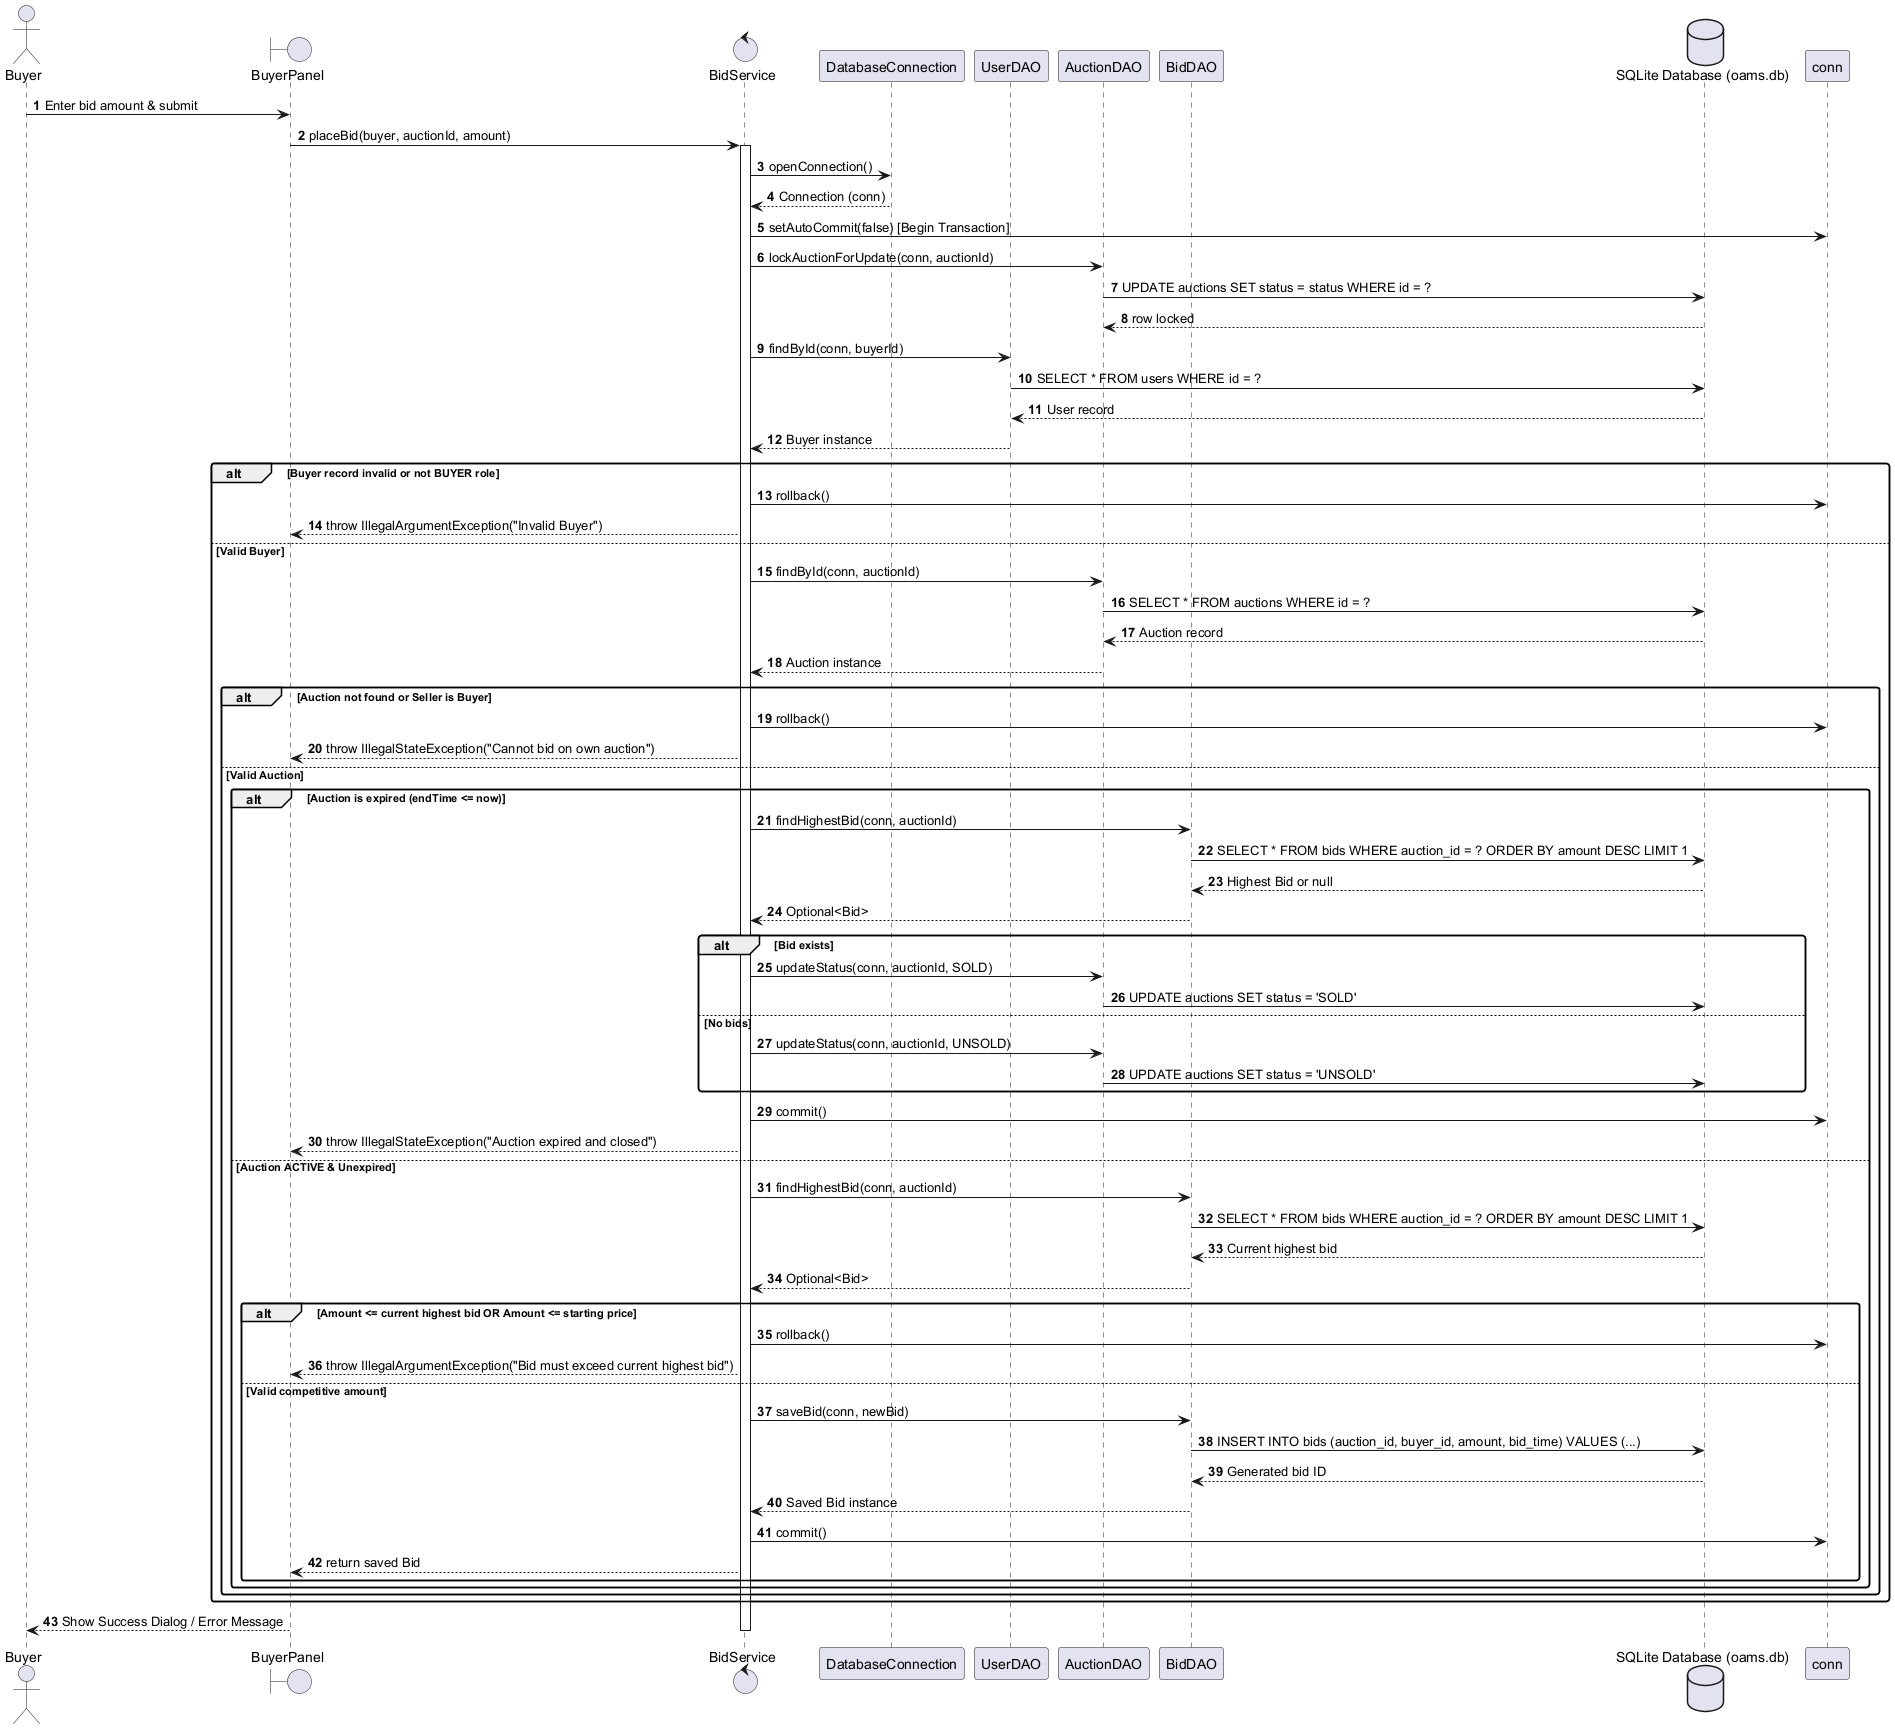
\includegraphics[width=0.98\textwidth]{figures/sequence_buyer_bid.png}
    \caption{UML Sequence Diagram: Transactional Bid Placement and Concurrency Locking}
    \label{fig:seq_bid}
\end{figure}

\paragraph{Step-by-Step Flow Analysis:}
\begin{enumerate}
    \item The Buyer inputs an amount in \texttt{BuyerPanel} and clicks ``Submit Bid''.
    \item \texttt{BuyerPanel} delegates to \texttt{BidService.placeBid(buyer, auctionId, amount)}.
    \item \texttt{BidService} obtains a JDBC connection and disables auto-commit (\texttt{setAutoCommit(false)}) to begin an ACID transaction.
    \item \texttt{BidService} calls \texttt{AuctionDAO.lockAuctionForUpdate(conn, auctionId)}, which issues a dummy update statement to acquire SQLite's reserved row/table lock.
    \item The buyer's persisted record is queried via \texttt{UserDAO.findById(conn, buyerId)} to verify that the buyer account exists and possesses the \texttt{BUYER} role. If invalid, the transaction rolls back.
    \item The target auction is fetched via \texttt{AuctionDAO.findById(conn, auctionId)}.
    \item \texttt{BidService} validates business rules:
    \begin{itemize}
        \item If the buyer is also the seller (\texttt{auction.getSellerId() == buyer.getId()}), the transaction is rolled back with an \texttt{IllegalStateException}.
        \item If the auction has expired (\texttt{now >= endTime}), \texttt{BidService} checks for existing bids. If present, status is updated to \texttt{SOLD}; otherwise, to \texttt{UNSOLD}. The transaction commits the status change, and the bid is rejected.
        \item If the auction is active and valid, \texttt{BidDAO.findHighestBid(conn, auctionId)} retrieves the current highest bid. If the submitted amount is less than or equal to the highest bid (or starting price), the transaction rolls back.
    \end{itemize}
    \item If all invariants pass, \texttt{BidDAO.saveBid(conn, bid)} inserts the new bid row.
    \item \texttt{BidService} commits the transaction (\texttt{conn.commit()}) and returns the persisted \texttt{Bid} object.
    \item \texttt{BuyerPanel} displays a success notification and refreshes bidding tables.
\end{enumerate}

\subsubsection{Scenario B: User Registration and Authentication}
Figure \ref{fig:seq_auth} illustrates user onboarding and authentication flows.

\begin{figure}[H]
    \centering
    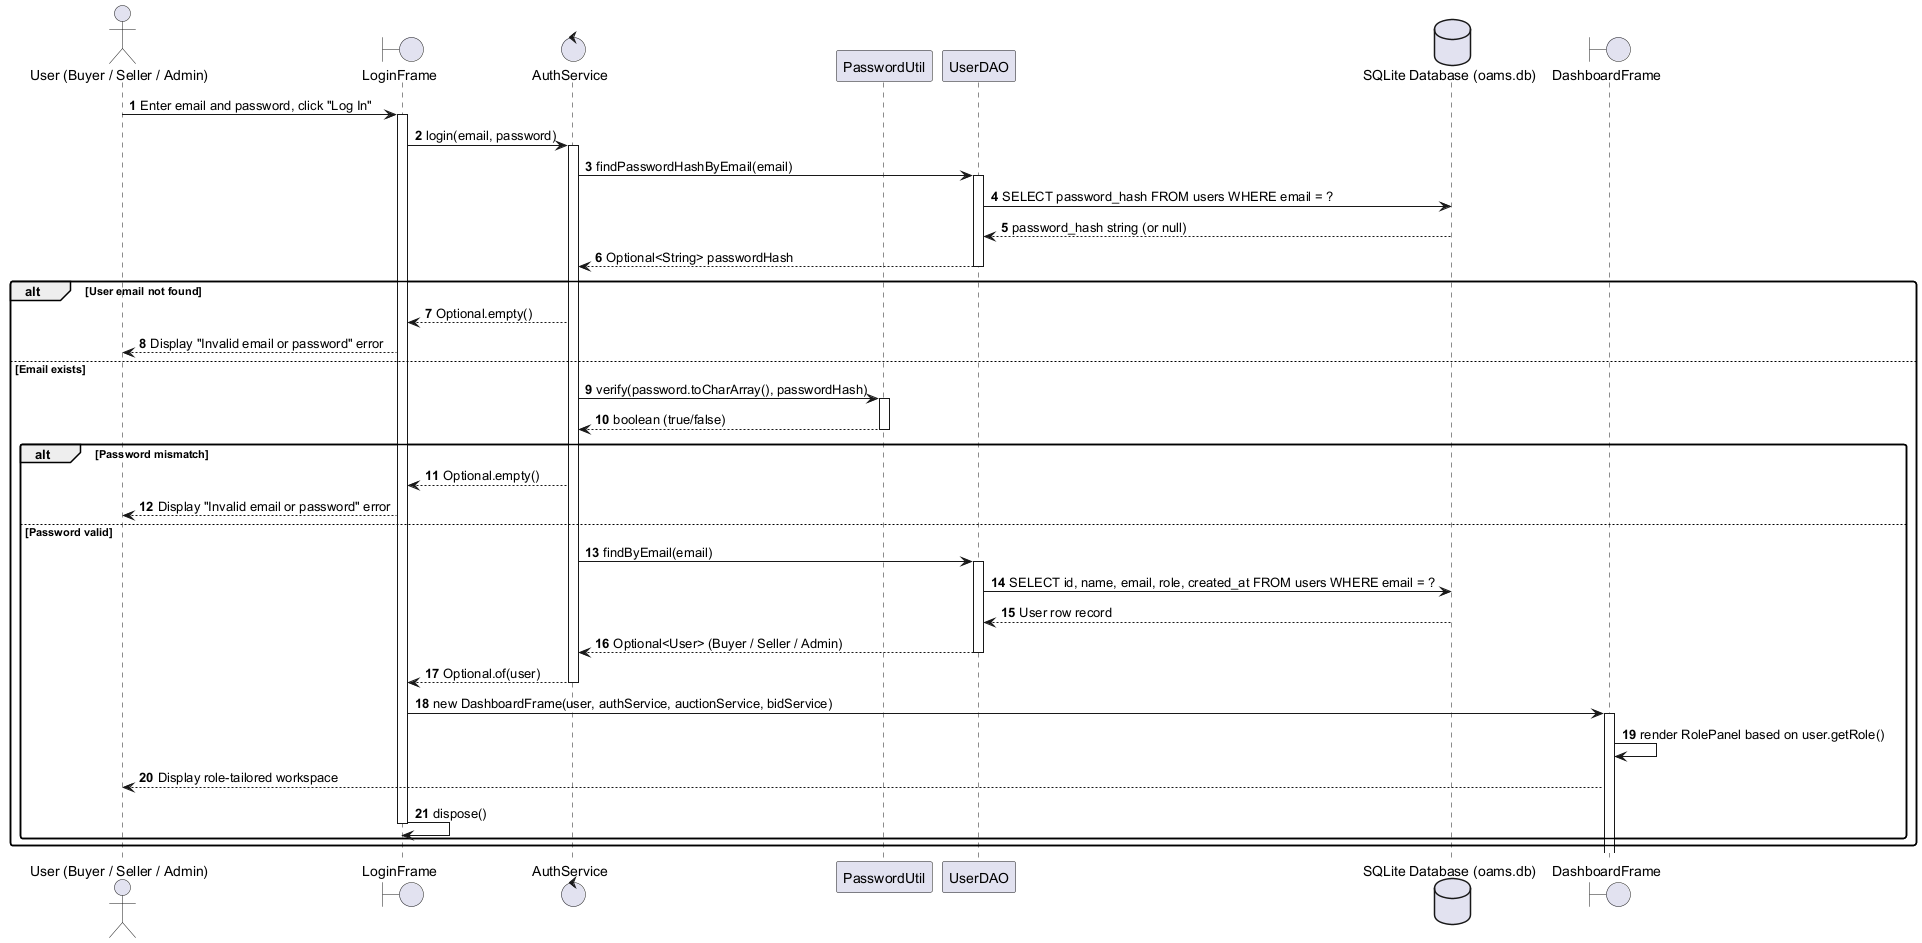
\includegraphics[width=0.95\textwidth]{figures/sequence_user_auth.png}
    \caption{UML Sequence Diagram: User Authentication and Dynamic Dashboard Initialization}
    \label{fig:seq_auth}
\end{figure}

\paragraph{Flow Analysis:}
The user enters credentials into \texttt{LoginFrame}, which forwards the request to \texttt{AuthService.login(email, password)}. The service queries \texttt{UserDAO.findPasswordHashByEmail(email)}. If a record exists, \texttt{PasswordUtil.verify(...)} evaluates the entered password against the stored PBKDF2 hash and salt. Upon verification, the user object is constructed from database fields and returned to \texttt{LoginFrame}, which disposes of itself and instantiates \texttt{DashboardFrame(user, ...)}. The dashboard inspects \texttt{user.getRole()} to render the appropriate workspace panel.

\subsubsection{Scenario C: Seller Creating an Auction}
Figure \ref{fig:seq_create} outlines the auction listing workflow.

\begin{figure}[H]
    \centering
    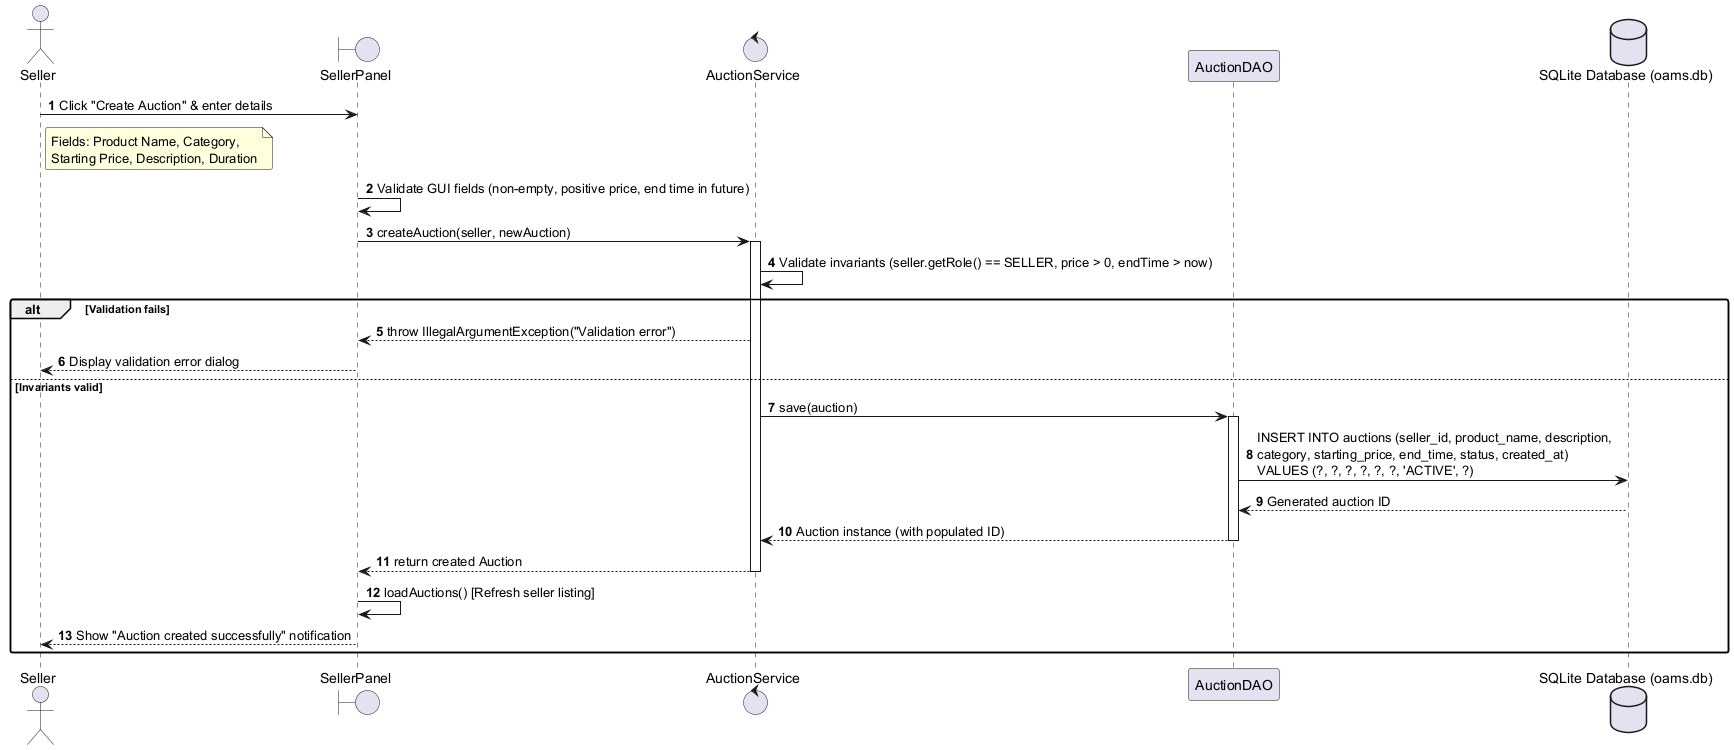
\includegraphics[width=0.90\textwidth]{figures/sequence_auction_create.png}
    \caption{UML Sequence Diagram: Seller Auction Listing Creation}
    \label{fig:seq_create}
\end{figure}

\paragraph{Flow Analysis:}
A Seller enters item details, starting price, and duration in \texttt{SellerPanel}. The panel constructs an \texttt{Auction} object, which enforces constructor validation (positive starting price, non-blank title). The panel calls \texttt{AuctionService.createAuction(seller, auction)}. The service verifies seller authorization, stamps the listing with \texttt{ACTIVE} status and creation timestamps, and delegates persistence to \texttt{AuctionDAO.save(auction)}. Upon successful insertion, the newly generated auction ID is returned, and the seller table refreshes automatically.

\subsubsection{Scenario D: Auction Closing and Winner Determination}
Figure \ref{fig:seq_close} depicts the automated lifecycle evaluation mechanism.

\begin{figure}[H]
    \centering
    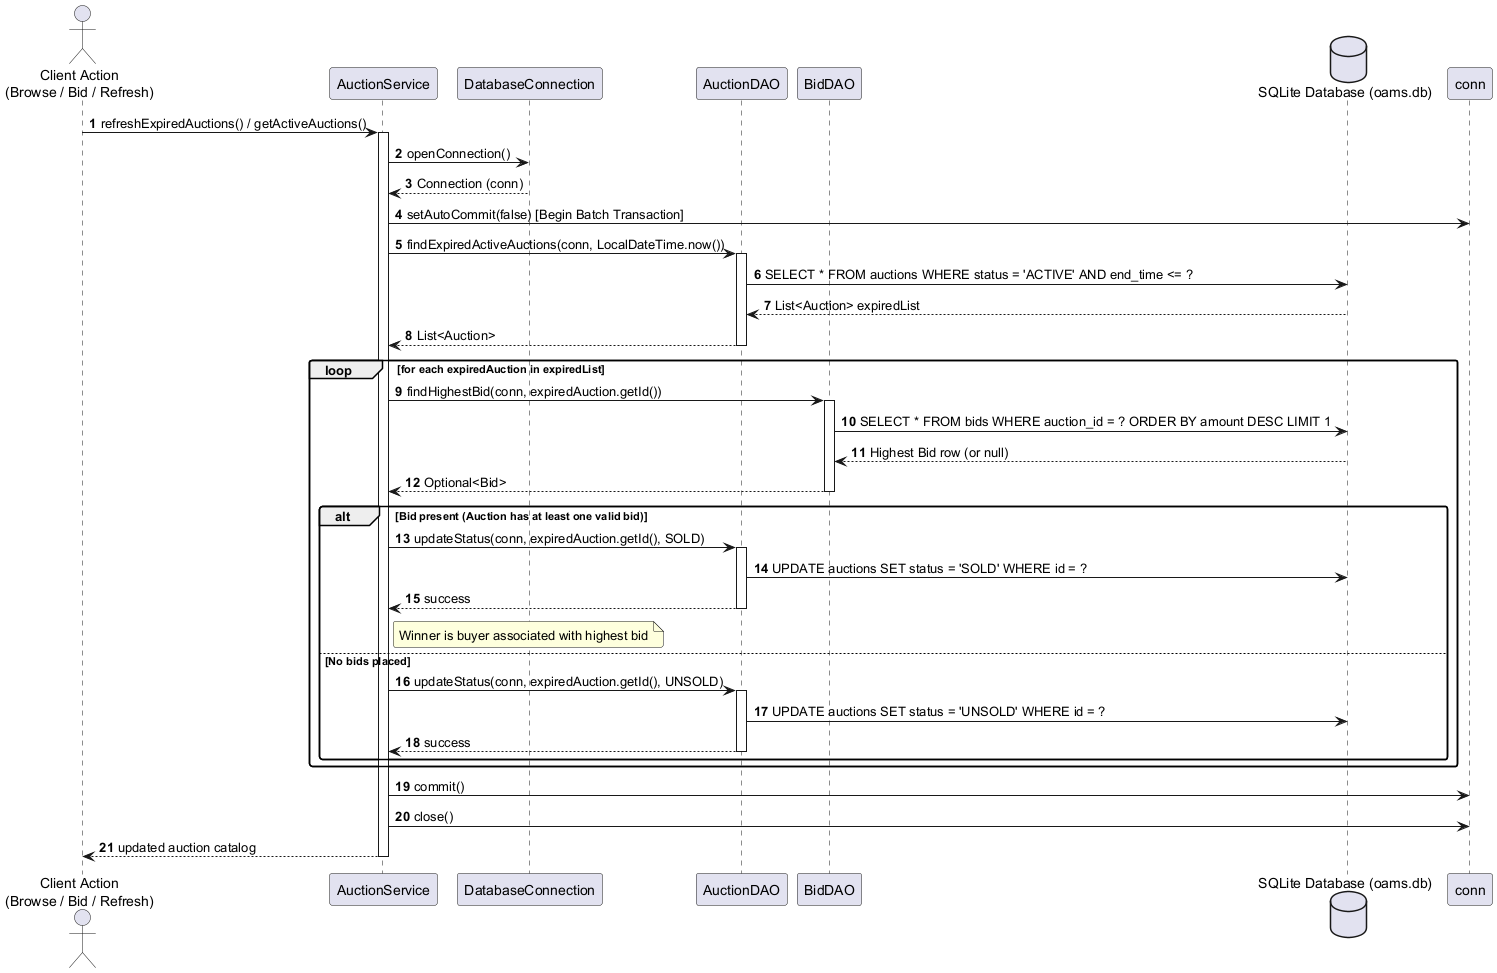
\includegraphics[width=0.95\textwidth]{figures/sequence_auction_close.png}
    \caption{UML Sequence Diagram: Lazy Auction Closing and Winner Settlement}
    \label{fig:seq_close}
\end{figure}

\paragraph{Flow Analysis:}
Auction settlement is evaluated on demand via a \textit{lazy expiration pattern}. Whenever an active catalog is requested or a bid is placed, \texttt{AuctionService.refreshExpiredAuctions()} executes. Within an ACID transaction, \texttt{AuctionDAO.findExpiredActiveAuctions(conn, now)} queries listings whose \texttt{end\_time} is in the past. For each expired listing:
\begin{itemize}
    \item If \texttt{BidDAO.findHighestBid(conn, auctionId)} returns a bid, the auction transitions to \texttt{SOLD}, establishing the highest bidder as the winner.
    \item If no bids exist, the auction transitions to \texttt{UNSOLD}.
\end{itemize}
The batch transaction is committed, ensuring catalog consistency without requiring an external scheduling process.

\subsubsection{Scenario E: Administrator Cancelling an Auction}
Figure \ref{fig:seq_cancel} models administrative listing moderation.

\begin{figure}[H]
    \centering
    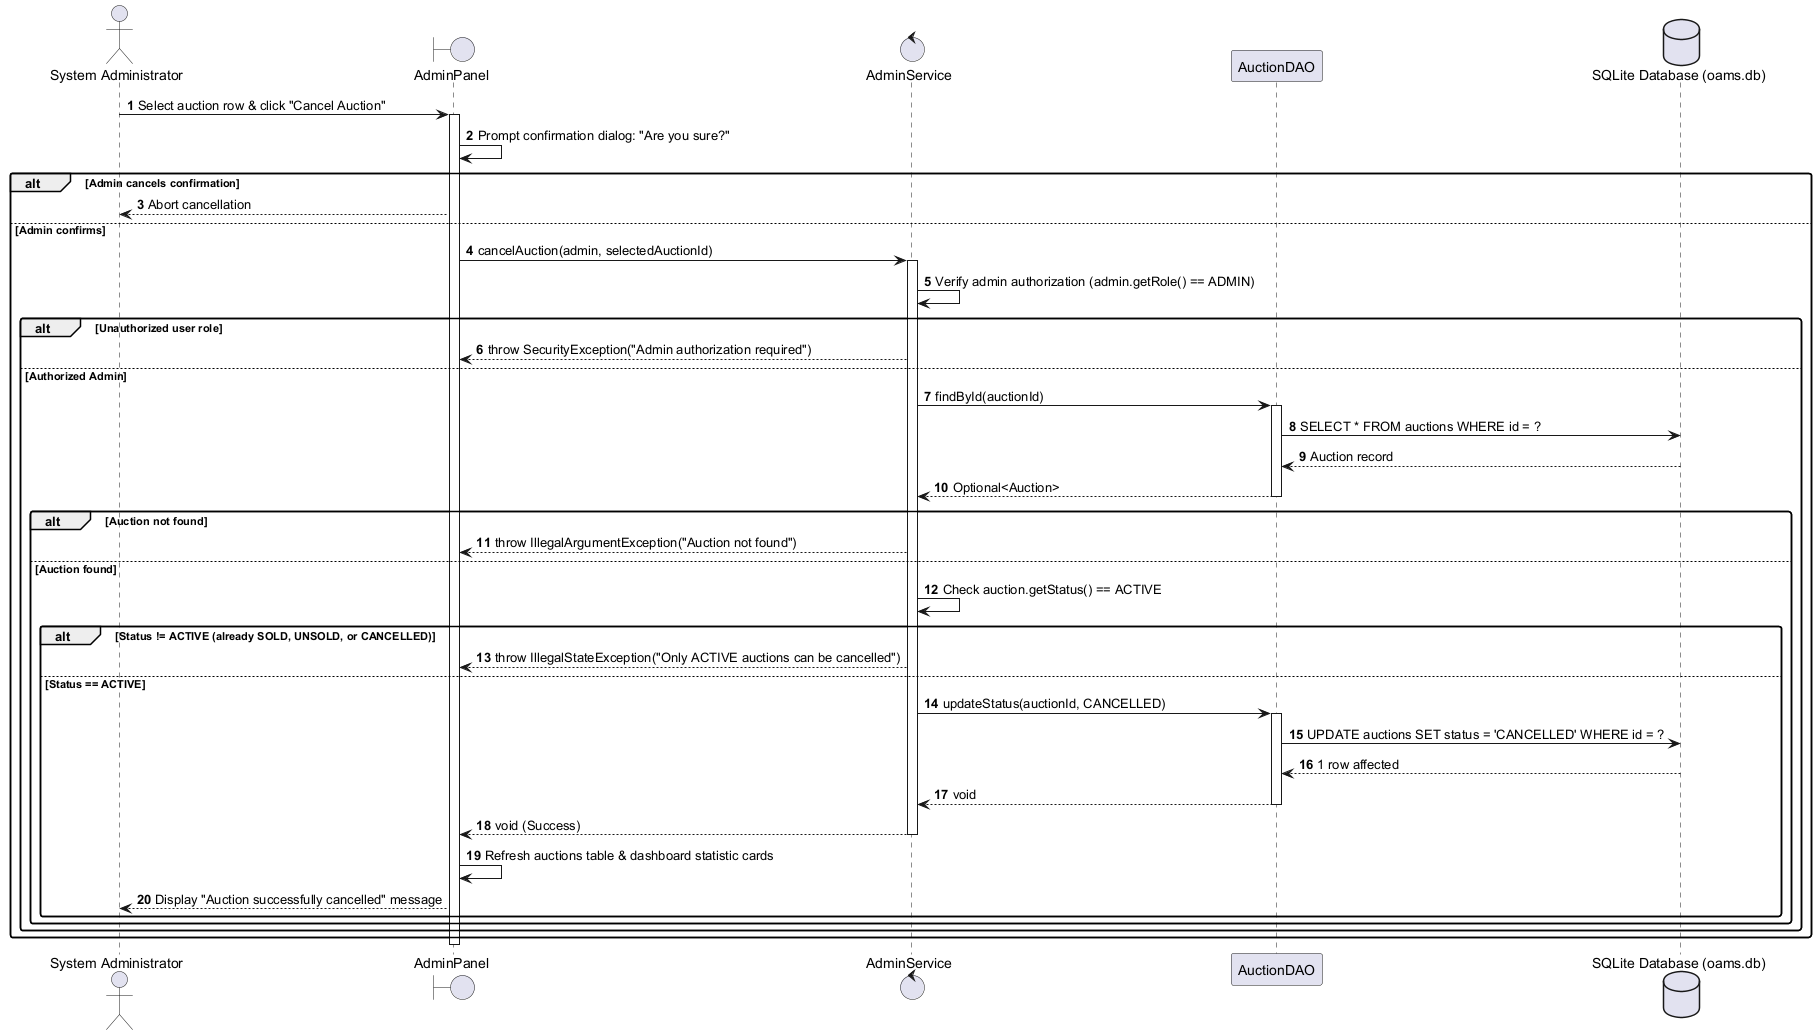
\includegraphics[width=0.95\textwidth]{figures/sequence_admin_cancel.png}
    \caption{UML Sequence Diagram: Administrative Auction Moderation and Cancellation}
    \label{fig:seq_cancel}
\end{figure}

\paragraph{Flow Analysis:}
An Administrator selects an auction in the Admin Panel and clicks ``Cancel Auction''. A confirmation dialog prompts for verification. Upon confirmation, \texttt{AdminService.cancelAuction(admin, auctionId)} is invoked. The service verifies that the invoking user possesses the \texttt{ADMIN} role and confirms via \texttt{AuctionDAO.findById(auctionId)} that the auction is currently in the \texttt{ACTIVE} state. If the auction is already \texttt{SOLD}, \texttt{UNSOLD}, or \texttt{CANCELLED}, the operation is rejected. Otherwise, \texttt{AuctionDAO.updateStatus(auctionId, CANCELLED)} updates the status. The Admin Panel then refreshes the auction table and updates dashboard metrics.

% ==============================================================================
% 4. ACTIVITY DIAGRAM
% ==============================================================================
\subsection{Activity Diagram (Workflow and Decision Logic)}
\label{subsec:uml_activity}

\subsubsection{Diagram Visualization}
Figure \ref{fig:activity_diagram} captures the end-to-end control flow of user interactions across different roles.

\begin{figure}[H]
    \centering
    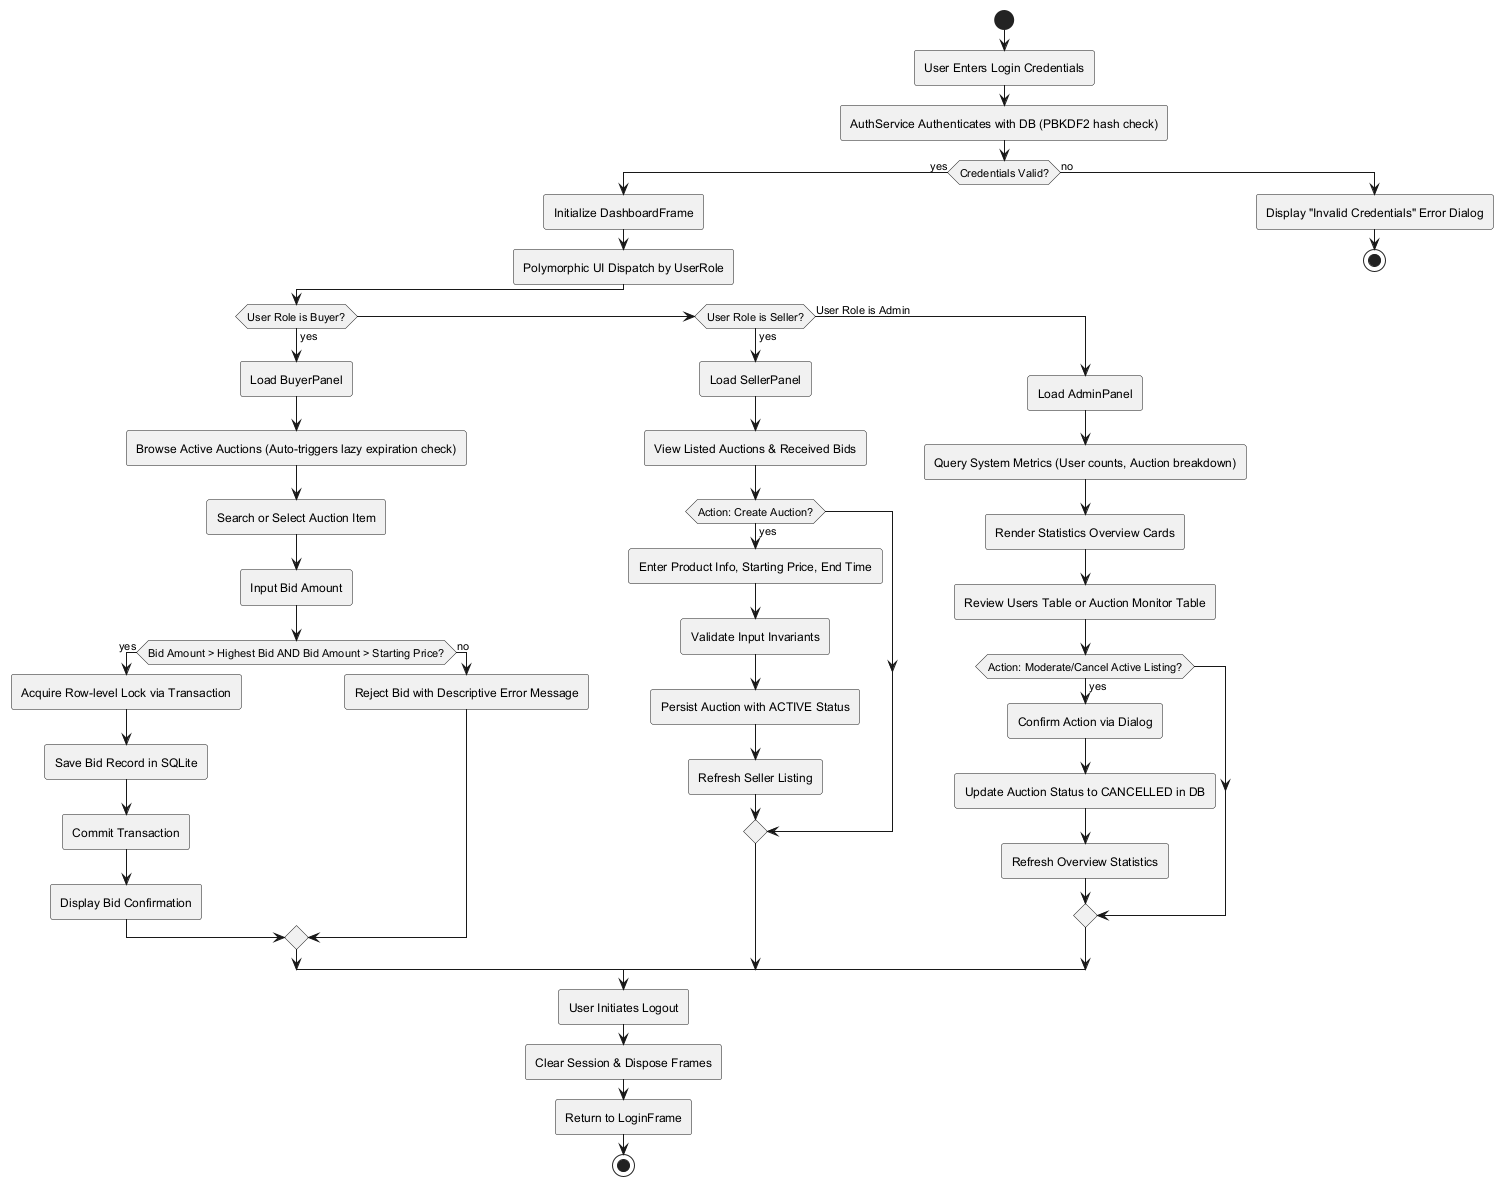
\includegraphics[width=0.85\textwidth]{figures/activity_diagram.png}
    \caption{UML Activity Diagram: End-to-End System Workflow and Decision Logic}
    \label{fig:activity_diagram}
\end{figure}

\subsubsection{Workflow Analysis}
The Activity diagram highlights conditional branching and concurrency controls:
\begin{enumerate}
    \item \textbf{Authentication Branching:} Credentials undergo hash validation. Failure routes to an error notification and halts the session; success branches into polymorphic role dashboards.
    \item \textbf{Buyer Bidding Path:} Includes active auction browsing, lazy expiration evaluation, bid amount comparison, transactional row locking, and database updates.
    \item \textbf{Seller Path:} Supports auction creation with invariant validation and tracking of received bids.
    \item \textbf{Admin Path:} Provides live metric queries, multi-criteria filtering, and listing moderation.
\end{enumerate}

% ==============================================================================
% 5. STATE MACHINE DIAGRAM
% ==============================================================================
\subsection{State Machine Diagram (Auction Entity Lifecycle)}
\label{subsec:uml_state_machine}

\subsubsection{Diagram Visualization}
Figure \ref{fig:state_machine} presents the finite state machine governing an \texttt{Auction} entity throughout its operational lifecycle.

\begin{figure}[H]
    \centering
    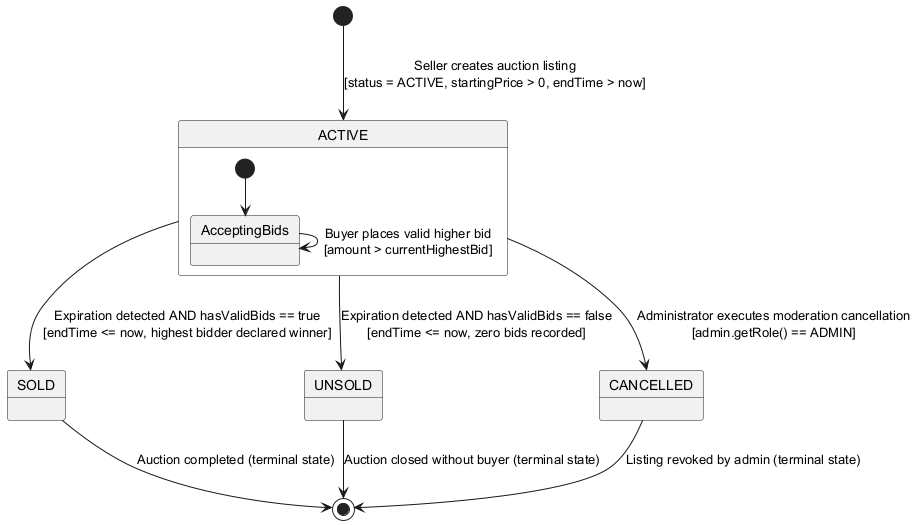
\includegraphics[width=0.85\textwidth]{figures/state_machine_diagram.png}
    \caption{UML State Machine Diagram for the \texttt{Auction} Entity}
    \label{fig:state_machine}
\end{figure}

\subsubsection{State Transitions and Guard Conditions}
An auction listing transitions through well-defined lifecycle states:
\begin{itemize}
    \item \textbf{Initial State $\rightarrow$ \texttt{ACTIVE}:} Transition occurs upon valid auction creation by an authenticated Seller with positive starting price and future end time.
    \item \textbf{\texttt{ACTIVE} Internal State (Accepting Bids):} While in \texttt{ACTIVE}, the auction receives bids. Each valid bid updates the prevailing highest price.
    \item \textbf{\texttt{ACTIVE} $\rightarrow$ \texttt{SOLD}:} Triggered when \texttt{now $\ge$ endTime} and \texttt{hasValidBids == true}. The highest bidder is declared the winner.
    \item \textbf{\texttt{ACTIVE} $\rightarrow$ \texttt{UNSOLD}:} Triggered when \texttt{now $\ge$ endTime} and \texttt{hasValidBids == false}. The listing terminates without sale.
    \item \textbf{\texttt{ACTIVE} $\rightarrow$ \texttt{CANCELLED}:} Triggered when an Administrator moderates an active listing.
    \item \textbf{Terminal States:} \texttt{SOLD}, \texttt{UNSOLD}, and \texttt{CANCELLED} are terminal states; no further transitions or bid submissions are permitted.
\end{itemize}

% ==============================================================================
% 6. COMPONENT DIAGRAM
% ==============================================================================
\subsection{Component Diagram (Structural Decomposition)}
\label{subsec:uml_component}

\subsubsection{Diagram Visualization}
Figure \ref{fig:component_diagram} models the modular software components and their interface dependencies.

\begin{figure}[H]
    \centering
    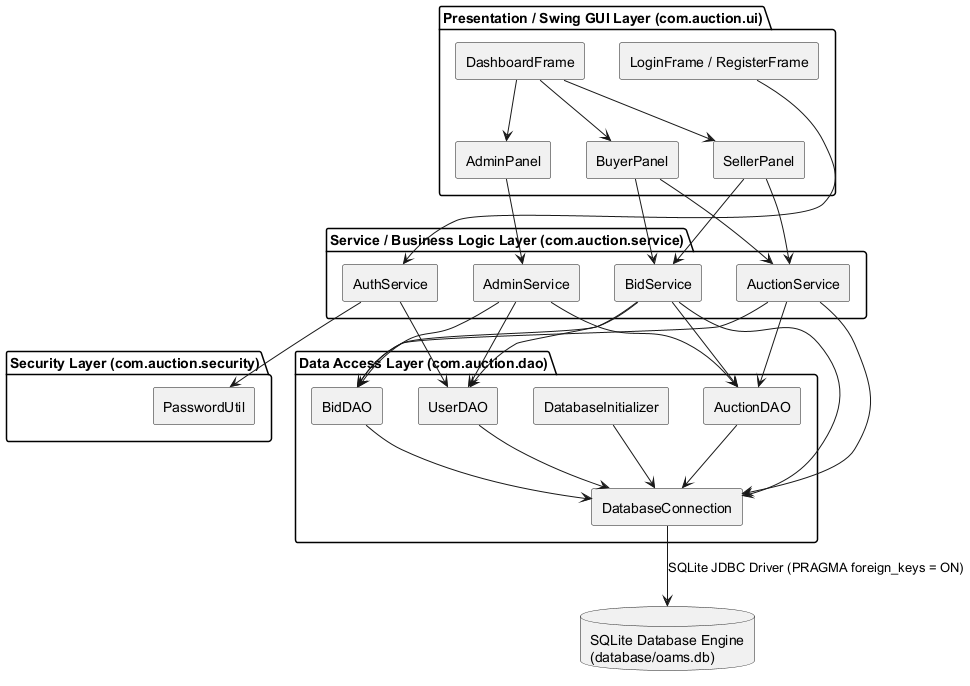
\includegraphics[width=0.92\textwidth]{figures/component_diagram.png}
    \caption{UML Component Diagram: Architectural Tiers and Inter-Component Dependencies}
    \label{fig:component_diagram}
\end{figure}

\subsubsection{Component Architecture}
The software is organized into four distinct architectural layers:
\begin{itemize}
    \item \textbf{Presentation Component:} Houses Swing frames and panels (\texttt{LoginFrame}, \texttt{DashboardFrame}, \texttt{BuyerPanel}, \texttt{SellerPanel}, \texttt{AdminPanel}).
    \item \textbf{Service Component:} Encapsulates business logic and orchestration (\texttt{AuthService}, \texttt{AuctionService}, \texttt{BidService}, \texttt{AdminService}).
    \item \textbf{Security Component:} Isolates cryptographic routines (\texttt{PasswordUtil}).
    \item \textbf{Data Access Component:} Encapsulates persistence logic and JDBC interactions (\texttt{UserDAO}, \texttt{AuctionDAO}, \texttt{BidDAO}, \texttt{DatabaseConnection}).
\end{itemize}

% ==============================================================================
% 7. DEPLOYMENT DIAGRAM
% ==============================================================================
\subsection{Deployment Diagram (Hardware and Runtime Environment)}
\label{subsec:uml_deployment}

\subsubsection{Diagram Visualization}
Figure \ref{fig:deployment_diagram} details the physical runtime environment and artifact deployment.

\begin{figure}[H]
    \centering
    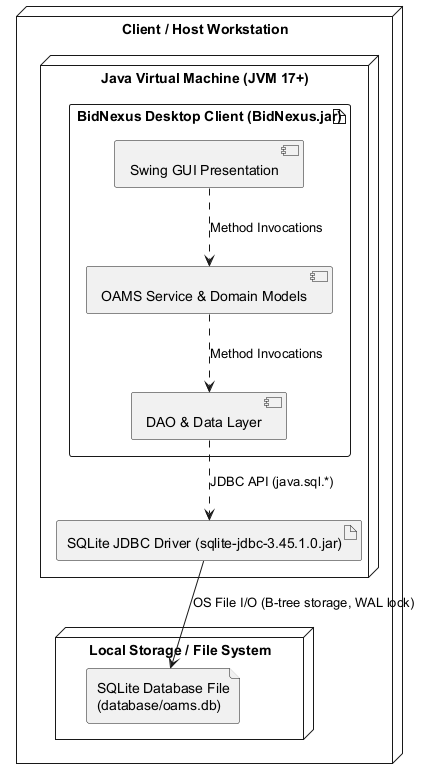
\includegraphics[width=0.85\textwidth]{figures/deployment_diagram.png}
    \caption{UML Deployment Diagram: Client Workstation Runtime Environment}
    \label{fig:deployment_diagram}
\end{figure}

\subsubsection{Deployment Architecture}
The system deploys as a standalone desktop application on a client workstation:
\begin{itemize}
    \item \textbf{Host Machine:} Any modern operating system (Windows, Linux, macOS) equipped with a Java Virtual Machine (JVM, JDK 17+).
    \item \textbf{Application Artifact:} The executable JAR file (\texttt{BidNexus.jar}), packaging presentation, service, and data access components.
    \item \textbf{Database Driver:} The SQLite JDBC Driver library (\texttt{sqlite-jdbc-3.45.1.0.jar}) embedded within the classpath.
    \item \textbf{Database Storage:} A local database file (\texttt{database/oams.db}), managed through filesystem file I/O with ACID transactional semantics.
\end{itemize}

% ==============================================================================
% 8. ENTITY-RELATIONSHIP (ER) DIAGRAM
% ==============================================================================
\subsection{Entity-Relationship (ER) Diagram (Relational Data Model)}
\label{subsec:uml_er}

\subsubsection{Diagram Visualization}
Figure \ref{fig:er_diagram} presents the Entity-Relationship model corresponding to the SQLite relational schema.

\begin{figure}[H]
    \centering
    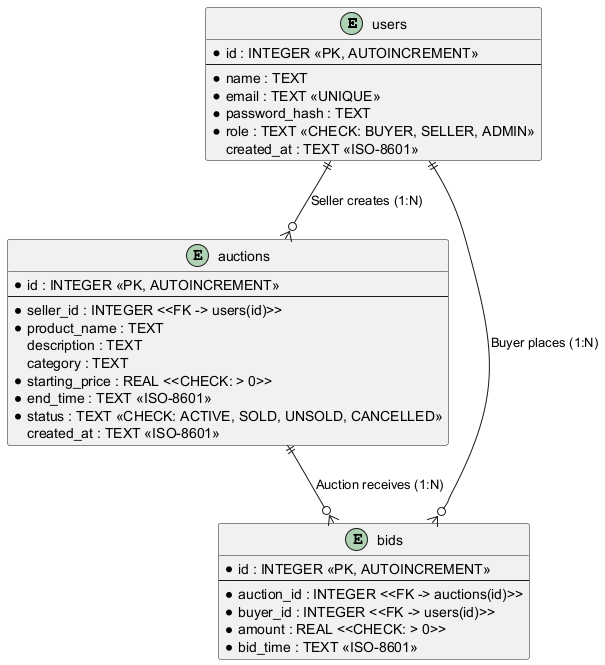
\includegraphics[width=0.88\textwidth]{figures/er_diagram.png}
    \caption{Entity-Relationship (ER) Diagram of the SQLite Relational Schema}
    \label{fig:er_diagram}
\end{figure}

\subsubsection{Entities, Attributes, and Cardinalities}
The database schema consists of three core relational tables:
\begin{itemize}
    \item \textbf{\texttt{users} Entity:} Stores user profiles. Attributes include \texttt{id} (PK), \texttt{name}, \texttt{email} (Unique), \texttt{password\_hash}, \texttt{role} (CHECK constraint), and \texttt{created\_at}.
    \item \textbf{\texttt{auctions} Entity:} Stores auction listings. Attributes include \texttt{id} (PK), \texttt{seller\_id} (FK referencing \texttt{users.id}), \texttt{product\_name}, \texttt{description}, \texttt{category}, \texttt{starting\_price} (CHECK $> 0$), \texttt{end\_time}, \texttt{status} (CHECK constraint), and \texttt{created\_at}.
    \item \textbf{\texttt{bids} Entity:} Stores bid transactions. Attributes include \texttt{id} (PK), \texttt{auction\_id} (FK referencing \texttt{auctions.id}), \texttt{buyer\_id} (FK referencing \texttt{users.id}), \texttt{amount} (CHECK $> 0$), and \texttt{bid\_time}.
    \item \textbf{Cardinalities:}
    \begin{itemize}
        \item One Seller can create zero or more Auctions ($1:N$).
        \item One Auction can receive zero or more Bids ($1:N$).
        \item One Buyer can place zero or more Bids ($1:N$).
    \end{itemize}
\end{itemize}
All foreign keys are strictly enforced at runtime via SQLite's foreign key pragma.

\newpage
\section{System Architecture and Design Patterns}
\label{sec:architecture}

\subsection{Architectural Overview}
Software architecture defines the fundamental organization of a system, embodied in its components, their relationships to one another and the environment, and the principles guiding its design and evolution \cite{martin2017clean, pressman2014software}. The Online Auction Management System (BidNexus) employs a \textbf{Multi-Tier Layered Architecture} structured according to the classic Separation of Concerns (SoC) principle.

Figure \ref{fig:arch_layers} conceptually models the flow of control and data dependencies across the four primary tiers.

\begin{figure}[H]
    \centering
    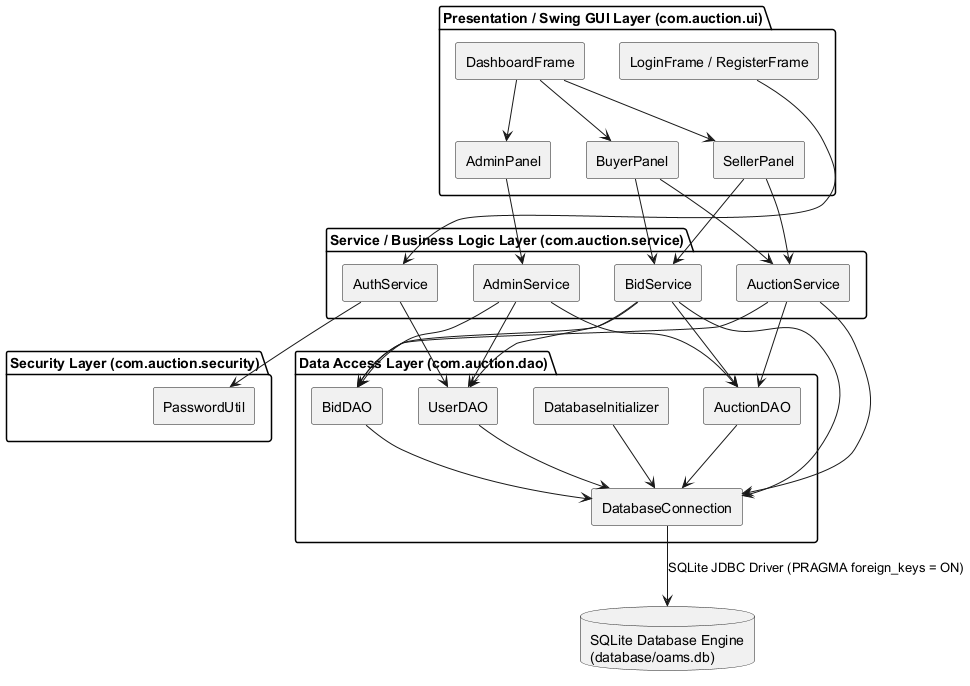
\includegraphics[width=0.88\textwidth]{figures/component_diagram.png}
    \caption{Layered Architectural Organization of BidNexus}
    \label{fig:arch_layers}
\end{figure}

\subsection{Detailed Tier Breakdown}

\subsubsection{1. Presentation Layer (Java Swing GUI)}
The presentation tier encapsulates all user interface rendering, user input capture, and visual feedback. It is housed in the \texttt{com.auction.ui} package. Key components include:
\begin{itemize}
    \item \texttt{LoginFrame} and \texttt{RegisterFrame}: Manage initial credential entry, user role selection, input validation, and delegation to the authentication service.
    \item \texttt{DashboardFrame}: The primary top-level window. Implements role-based dynamic workspace provisioning, rendering customized sidebars and views based on the authenticated user's polymorphic role.
    \item \texttt{BuyerPanel}: Provides auction browsing, keyword search filtering, modal bidding dialogs, and tabular views for ``My Bids'' and ``Auction Results''.
    \item \texttt{SellerPanel}: Provides listing creation dialogs, inventory status monitoring, and itemized bid history tables for seller listings.
    \item \texttt{AdminPanel}: Provides system-wide dashboard metric cards, multi-field user search, auction monitoring, and modal cancellation confirmation dialogs.
    \item \texttt{UiStyle}: A centralized presentation utility that provides consistent color palettes, typography (Segoe UI), card borders, and UI component factories.
\end{itemize}

A critical architectural rule of this layer is that GUI components \textbf{never execute SQL queries or hold direct JDBC references}. All database interactions are delegated through the Service Layer.

\subsubsection{2. Service Layer (Business Logic and Policy Orchestration)}
The service tier, located in \texttt{com.auction.service}, encapsulates business rules, policy constraints, workflow coordination, and transaction management:
\begin{itemize}
    \item \texttt{AuthService}: Orchestrates user onboarding, ensures email uniqueness, invokes password hashing routines, and verifies credentials during login.
    \item \texttt{AuctionService}: Enforces listing policies (e.g., positive reserve prices, future expiration dates), coordinates catalog queries, and conducts lazy expiration sweeps.
    \item \texttt{BidService}: Coordinates competitive bidding, implements row-level locking for concurrency protection, enforces anti-shill policies (blocking sellers from bidding on their own listings), and determines auction winners.
    \item \texttt{AdminService}: Aggregates cross-table platform metrics, coordinates multi-criteria user and auction searches, and validates administrative moderation policies.
\end{itemize}

\subsubsection{3. Security Layer (Cryptographic Utilities)}
The security tier, isolated in \texttt{com.auction.security}, houses \texttt{PasswordUtil}. This utility implements PBKDF2 with HMAC-SHA256, generating unique cryptographically secure 16-byte salts and 256-bit derived hashes with 65,536 iterations. Model objects never store or expose password hashes, adhering to the principle of least privilege.

\subsubsection{4. Data Access Layer (DAO and Persistence)}
The persistence tier, situated in \texttt{com.auction.dao}, encapsulates all SQL query formulation, execution, and Object-Relational mapping:
\begin{itemize}
    \item \texttt{DatabaseConnection}: Manages SQLite JDBC connection lifecycles, ensures the database directory exists, and enforces foreign key support via \texttt{PRAGMA foreign\_keys = ON}.
    \item \texttt{UserDAO}, \texttt{AuctionDAO}, \texttt{BidDAO}: Implement CRUD operations using parameterized \texttt{PreparedStatement} objects. Overloaded methods support both auto-closing standalone connections and caller-managed connections for multi-step transactions.
    \item \texttt{DatabaseInitializer}: Executes schema creation DDL scripts with \texttt{CREATE TABLE IF NOT EXISTS} statements.
\end{itemize}

\subsubsection{5. Relational Database Layer (SQLite)}
The foundational storage engine is SQLite 3, embedded locally at \texttt{database/oams.db}. SQLite provides lightweight, zero-configuration persistence with ACID transactional guarantees.

\subsection{Object-Oriented Design Patterns Applied}
BidNexus applies several classical design patterns to solve common architectural problems:

\paragraph{1. Data Access Object (DAO) Pattern \cite{gamma1994design}:}
The DAO pattern abstracts and encapsulates all access to the database. By providing explicit interfaces (\texttt{UserDAO}, \texttt{AuctionDAO}, \texttt{BidDAO}), the rest of the application remains completely decoupled from SQLite-specific dialect nuances.

\paragraph{2. Model-View-Controller (MVC) Idiom:}
The application adheres to MVC principles within Java Swing:
\begin{itemize}[noitemsep]
    \item \textbf{Model:} Domain entities (\texttt{User}, \texttt{Auction}, \texttt{Bid}) represent application state.
    \item \textbf{View:} Swing panels and frames render data into tables and cards.
    \item \textbf{Controller:} Service classes and action listeners process user input, mutate state, and trigger UI updates.
\end{itemize}

\paragraph{3. Dependency Injection (Constructor Injection):}
Classes receive their dependencies through constructor arguments rather than instantiating them internally. For example, \texttt{BidService} accepts \texttt{DatabaseConnection}, \texttt{AuctionDAO}, \texttt{BidDAO}, and \texttt{UserDAO}. This decouples components and facilitates automated unit testing using temporary in-memory database instances.

\paragraph{4. Immutable Domain Entity Pattern \cite{bloch2018effective}:}
Domain models are constructed as immutable objects with \texttt{private final} fields and no setters. This prevents unintentional mutation and ensures thread-safe data transfer across UI and service layers.

\subsection{Cross-Layer Data Flow}
Figure \ref{fig:data_flow_trace} illustrates how a user action traverses the architectural tiers during a bid submission.

\begin{figure}[H]
    \centering
    \begin{minipage}{0.95\textwidth}
        \centering
        \fbox{
        \parbox{0.9\textwidth}{
        \centering
        \vspace{0.2cm}
        \textbf{Presentation Tier (\texttt{BuyerPanel})}\\[0.1cm]
        Captures bid amount $\rightarrow$ Validates numeric format $\rightarrow$ Calls \texttt{BidService.placeBid()}\\[0.2cm]
        $\boldsymbol{\downarrow}$\\[0.2cm]
        \textbf{Service Tier (\texttt{BidService})}\\[0.1cm]
        Opens JDBC connection $\rightarrow$ Begins Transaction (\texttt{setAutoCommit(false)}) $\rightarrow$\\
        Executes Row Lock $\rightarrow$ Verifies Invariants (Eligibility, Status, Expiration, Amount)\\[0.2cm]
        $\boldsymbol{\downarrow}$\\[0.2cm]
        \textbf{Data Access Tier (\texttt{BidDAO} \& \texttt{AuctionDAO})}\\[0.1cm]
        Executes Parameterized SQL: \texttt{INSERT INTO bids ...} $\rightarrow$ Maps result to \texttt{Bid} entity\\[0.2cm]
        $\boldsymbol{\downarrow}$\\[0.2cm]
        \textbf{Database Engine (SQLite)}\\[0.1cm]
        Validates CHECK and FK constraints $\rightarrow$ Writes to disk/WAL $\rightarrow$ Acknowledges Commit\\[0.2cm]
        $\boldsymbol{\downarrow}$\\[0.2cm]
        \textbf{Return Path: Service commits $\rightarrow$ Returns \texttt{Bid} $\rightarrow$ GUI updates table and displays confirmation}
        \vspace{0.2cm}
        }
        }
        \caption{End-to-End Control and Data Flow Trace for Bid Placement}
        \label{fig:data_flow_trace}
    \end{minipage}
\end{figure}

\newpage
\section{Technology Stack and Engineering Tools}
\label{sec:technology_stack}

\subsection{Technology Selection Rationale}
The technical stack for the Online Auction Management System (BidNexus) was carefully chosen to balance educational clarity in Object-Oriented Methodologies with industry-standard development practices. Each framework and library was selected for stability, zero-overhead deployment, and native support for core object-oriented principles.

Table \ref{tab:tech_stack} summarizes the primary technologies, versions, and architectural roles within the project.

\begin{table}[H]
\centering
\small
\caption{Comprehensive Technology Stack Specification}
\label{tab:tech_stack}
\begin{tabularx}{\textwidth}{p{3cm}p{2cm}p{3cm}X}
\toprule
\textbf{Technology} & \textbf{Version} & \textbf{Category} & \textbf{Architectural Role and Justification} \\
\midrule
\textbf{Java Platform (JDK)} & 17+ (LTS) & Core Programming Language & Provides strong static typing, OOP abstractions, pattern matching, switch expressions, and modern date/time APIs (\texttt{java.time}). \\
\addlinespace
\textbf{Java Swing / AWT} & JDK Built-in & GUI Toolkit & Provides lightweight, cross-platform desktop UI components; predictable event handling on the Event Dispatch Thread (EDT). \\
\addlinespace
\textbf{SQLite} & 3.45+ & Relational Database & Embedded, serverless, zero-configuration relational storage engine providing ACID transactions and foreign key enforcement. \\
\addlinespace
\textbf{SQLite JDBC Driver} & 3.45.1.0 & Database Connectivity & Standard JDBC driver enabling connection management, prepared statements, and transactional commit/rollback control. \\
\addlinespace
\textbf{Apache Maven} & 3.9+ & Build and Dependency Management & Standardizes the build lifecycle, compiles source code, manages dependencies, and automates test suite execution. \\
\addlinespace
\textbf{JUnit 5 (Jupiter)} & 5.10.2 & Automated Testing Framework & Executes automated unit and integration tests; provides \texttt{@TempDir} for isolated file-based database testing. \\
\addlinespace
\textbf{PlantUML} & 1.2024+ & Visual UML Modeling & Text-based diagramming engine generating formal UML diagrams from declarative source code. \\
\bottomrule
\end{tabularx}
\end{table}

\subsection{In-Depth Component Evaluation}

\subsubsection{1. Java 17 Platform Features}
BidNexus leverages modern Java language enhancements that promote cleaner object-oriented design and reduce boilerplate code:
\begin{itemize}
    \item \textbf{Pattern Matching for \texttt{instanceof}:} Simplifies type interrogation and casting, enabling safe polymorphic branching in \texttt{DashboardFrame} (e.g., \texttt{if (user instanceof Buyer buyer)}).
    \item \textbf{Switch Expressions with Arrow Syntax:} Provides concise, exhaustiveness-checked pattern matching for role and status evaluation without falling-through risks.
    \item \textbf{\texttt{java.time} Framework:} Replaces legacy \texttt{java.util.Date} with immutable, thread-safe temporal types (\texttt{LocalDateTime}) for precise auction deadline evaluations.
    \item \textbf{\texttt{BigDecimal} for Financial Precision:} Eliminates IEEE 754 floating-point rounding errors during currency calculations and bid comparisons.
\end{itemize}

\subsubsection{2. Java Swing and Multithreaded UI Execution}
Java Swing was selected for the presentation tier because it ships natively with the JDK, eliminating external native UI dependencies. To maintain a responsive interface:
\begin{itemize}
    \item All UI mutations run strictly on the \textbf{Event Dispatch Thread (EDT)} via \texttt{SwingUtilities.invokeLater}.
    \item Long-running administrative database aggregations and search queries are offloaded to \texttt{SwingWorker} background threads, preventing UI freezing during heavy queries.
\end{itemize}

\subsubsection{3. Embedded SQLite and JDBC Integration}
Unlike enterprise RDBMS solutions (e.g., PostgreSQL or MySQL) that require running background server daemons and network socket configuration, SQLite is an \textit{embedded serverless} database. The entire database resides in a single cross-platform file (\texttt{database/oams.db}). This simplifies deployment and testing while still supporting standard SQL syntax, foreign key constraints, and transactional consistency.

Through the \texttt{sqlite-jdbc} driver, BidNexus configures SQLite for production-grade reliability:
\begin{itemize}[noitemsep]
    \item Foreign key checks are explicitly activated via \texttt{PRAGMA foreign\_keys = ON}.
    \item Transactions are controlled explicitly via \texttt{Connection.setAutoCommit(false)}, \texttt{commit()}, and \texttt{rollback()}.
\end{itemize}

\subsubsection{4. Apache Maven Build Lifecycle}
Maven manages the project build lifecycle, dependency resolution, and test execution. Listing \ref{lst:pom_excerpt} presents the core configuration from \texttt{pom.xml}.

\begin{lstlisting}[caption={Maven Build Configuration (\texttt{pom.xml})}, label={lst:pom_excerpt}]
<project xmlns="http://maven.apache.org/POM/4.0.0" ...>
    <modelVersion>4.0.0</modelVersion>
    <groupId>com.auction</groupId>
    <artifactId>online-auction-management-system</artifactId>
    <version>1.0-SNAPSHOT</version>

    <properties>
        <maven.compiler.source>17</maven.compiler.source>
        <maven.compiler.target>17</maven.compiler.target>
        <project.build.sourceEncoding>UTF-8</project.build.sourceEncoding>
        <junit.jupiter.version>5.10.2</junit.jupiter.version>
    </properties>

    <dependencies>
        <!-- Embedded SQLite JDBC Driver -->
        <dependency>
            <groupId>org.xerial</groupId>
            <artifactId>sqlite-jdbc</artifactId>
            <version>3.45.1.0</version>
        </dependency>
        <!-- JUnit 5 Testing Framework -->
        <dependency>
            <groupId>org.junit.jupiter</groupId>
            <artifactId>junit-jupiter</artifactId>
            <version>${junit.jupiter.version}</version>
            <scope>test</scope>
        </dependency>
    </dependencies>
</project>
\end{lstlisting}

\newpage
\section{System Implementation Details}
\label{sec:implementation}

\subsection{Implementation Overview}
The implementation of the Online Auction Management System (BidNexus) translates the object-oriented design and architectural specifications into robust, production-quality Java code. This chapter details the technical implementation across five core modules: Authentication and Cryptography, Auction Lifecycle and Lazy Expiration, Concurrency-Safe Bidding, Administrative Governance, and User Interface Engineering.

\subsection{Module 1: Authentication and Cryptographic Security}
Authentication is coordinated by \texttt{AuthService} in conjunction with \texttt{PasswordUtil}. To protect user credentials against rainbow table attacks and credential stuffing, passwords undergo cryptographic hashing prior to storage.

Listing \ref{lst:password_util} highlights the cryptographic implementation in \texttt{PasswordUtil.java}.

\begin{lstlisting}[caption={Cryptographic Hash Generation and Verification in \texttt{PasswordUtil.java}}, label={lst:password_util}]
public final class PasswordUtil {
    private static final String ALGORITHM = "PBKDF2WithHmacSHA256";
    private static final int ITERATIONS = 65536;
    private static final int KEY_LENGTH = 256;
    private static final int SALT_BYTES = 16;

    public static String hash(char[] password) {
        byte[] salt = new byte[SALT_BYTES];
        new SecureRandom().nextBytes(salt);
        byte[] hash = pbkdf2(password, salt, ITERATIONS, KEY_LENGTH);
        return Base64.getEncoder().encodeToString(salt) + ":" + 
               ITERATIONS + ":" + 
               Base64.getEncoder().encodeToString(hash);
    }

    public static boolean verify(char[] password, String storedHash) {
        String[] parts = storedHash.split(":");
        byte[] salt = Base64.getDecoder().decode(parts[0]);
        int iterations = Integer.parseInt(parts[1]);
        byte[] expectedHash = Base64.getDecoder().decode(parts[2]);
        byte[] actualHash = pbkdf2(password, salt, iterations, expectedHash.length * 8);
        return MessageDigest.isEqual(expectedHash, actualHash); // Constant-time comparison
    }
}
\end{lstlisting}

\paragraph{Key Security Decisions:}
\begin{enumerate}
    \item \textbf{Unique Cryptographic Salt:} A 16-byte cryptographically secure pseudo-random salt is generated per password.
    \item \textbf{High Iteration Work Factor:} 65,536 iterations increase the computational cost for brute-force attacks.
    \item \textbf{Constant-Time Verification:} \texttt{MessageDigest.isEqual} prevents timing side-channel attacks by comparing byte arrays in constant time.
    \item \textbf{No Password State in Models:} Model entities (\texttt{User}, \texttt{Buyer}, \texttt{Seller}) never store or expose password hashes.
\end{enumerate}

\subsection{Module 2: Auction Lifecycle and Lazy Expiration}
A recurring challenge in auction platforms is ensuring that auctions terminate precisely when their scheduled expiration timestamp arrives. Traditional implementations often rely on background timer threads (e.g., \texttt{ScheduledExecutorService}). However, in desktop and embedded contexts, timer threads can terminate unexpectedly if the application encounters an unhandled exception.

BidNexus implements a deterministic \textbf{Lazy Expiration Pattern}. Whenever an active catalog is queried or a bid is placed, \texttt{AuctionService.refreshExpiredAuctions()} executes automatically.

Listing \ref{lst:lazy_expiration} illustrates how expired listings are evaluated and resolved.

\begin{lstlisting}[caption={Deterministic Lazy Expiration in \texttt{AuctionService.java}}, label={lst:lazy_expiration}]
public void refreshExpiredAuctions() throws SQLException {
    LocalDateTime now = LocalDateTime.now();
    try (Connection conn = databaseConnection.openConnection()) {
        conn.setAutoCommit(false);
        try {
            List<Auction> expiredList = auctionDAO.findExpiredActiveAuctions(conn, now);
            for (Auction auction : expiredList) {
                boolean hasBids = bidDAO.findHighestBid(conn, auction.getId()).isPresent();
                AuctionStatus newStatus = hasBids ? AuctionStatus.SOLD : AuctionStatus.UNSOLD;
                auctionDAO.updateStatus(conn, auction.getId(), newStatus);
            }
            conn.commit();
        } catch (SQLException | RuntimeException ex) {
            conn.rollback();
            throw ex;
        }
    }
}
\end{lstlisting}

This approach guarantees that users never observe an expired auction in an \texttt{ACTIVE} state, ensuring accurate winner determination without requiring persistent background daemon processes.

\subsection{Module 3: Concurrency Control and Transactional Bidding}
Bidding is the most concurrency-sensitive operation in an auction system. If two buyers simultaneously bid on the same item, a race condition can cause the lower bid to overwrite the higher bid.

BidNexus solves this challenge in \texttt{BidService.placeBid()} by coordinating an ACID transaction with an explicit update lock in SQLite, as shown in Listing \ref{lst:bidding_transaction}.

\begin{lstlisting}[caption={ACID Transaction and Row-Level Locking in \texttt{BidService.java}}, label={lst:bidding_transaction}]
public Bid placeBid(Buyer buyer, int auctionId, double amount) throws SQLException {
    if (buyer == null || buyer.getId() <= 0) {
        throw new IllegalArgumentException("Sign in with a Buyer account before bidding");
    }
    BigDecimal bidAmount = BigDecimal.valueOf(amount);

    try (Connection connection = databaseConnection.openConnection()) {
        connection.setAutoCommit(false); // Begin ACID transaction
        try {
            // Acquire row-level lock via update statement
            lockAuctionForUpdate(connection, auctionId);

            User persistedBuyer = userDAO.findById(connection, buyer.getId())
                    .orElseThrow(() -> new IllegalArgumentException("Buyer account invalid"));
            if (!(persistedBuyer instanceof Buyer)) {
                throw new IllegalArgumentException("Only registered Buyers can place bids");
            }

            Auction auction = auctionDAO.findById(connection, auctionId)
                    .orElseThrow(() -> new IllegalArgumentException("Auction was not found"));
            if (auction.getStatus() != AuctionStatus.ACTIVE) {
                throw new IllegalArgumentException("This auction is not accepting bids");
            }
            if (auction.getSellerId() == buyer.getId()) {
                throw new IllegalArgumentException("You cannot bid on your own auction");
            }

            LocalDateTime now = LocalDateTime.now();
            if (auction.isExpired(now)) {
                AuctionStatus expiredStatus = bidDAO.findHighestBid(connection, auctionId).isPresent()
                        ? AuctionStatus.SOLD : AuctionStatus.UNSOLD;
                auctionDAO.updateStatus(connection, auctionId, expiredStatus);
                connection.commit();
                throw new IllegalStateException("Auction expired and is now closed");
            }

            BigDecimal currentPrice = bidDAO.findHighestBid(connection, auctionId)
                    .map(Bid::getAmount)
                    .orElse(auction.getStartingPrice());
            if (bidAmount.compareTo(currentPrice) <= 0) {
                throw new IllegalArgumentException("Bid must exceed current price of " + currentPrice);
            }

            Bid savedBid = bidDAO.saveBid(connection, 
                new Bid(0, auctionId, buyer.getId(), bidAmount, now));
            connection.commit(); // Atomic commit
            return savedBid;
        } catch (SQLException | RuntimeException exception) {
            connection.rollback(); // Rollback on any failure
            throw exception;
        }
    }
}
\end{lstlisting}

\subsection{Module 4: Administrative Governance and Panel Implementation}
The administrative subsystem provides real-time system monitoring, auditing, and moderation:
\begin{enumerate}
    \item \textbf{Live Dashboard Statistics:} \texttt{AdminService.getDashboardOverview()} executes optimized SQL aggregation queries to compute live counts for total users, buyers, sellers, admins, total auctions, active auctions, sold auctions, unsold auctions, and cancelled auctions.
    \item \textbf{Multi-Criteria User and Auction Search:} \texttt{AdminPanel} provides combined keyword search fields and role/status dropdown filters, enabling administrators to locate users or auctions by ID, name, email, or lifecycle status.
    \item \textbf{Detailed Modal Dialogs:} Selecting any row in the users or auctions table enables a ``View Details'' action that opens an informative modal dialog displaying complete entity attributes and itemized bidding logs.
    \item \textbf{Policy-Compliant Auction Cancellation:} Administrators can cancel an active auction. As implemented in \texttt{AdminService.cancelAuction()}, the system checks that the user has the \texttt{ADMIN} role and confirms the target listing is currently \texttt{ACTIVE}. If the auction is already \texttt{SOLD}, \texttt{UNSOLD}, or \texttt{CANCELLED}, the system throws an \texttt{IllegalStateException}, preventing modification of finalized commercial records.
\end{enumerate}

\subsection{Module 5: Swing GUI Layout and Asynchronous UI Execution}
To prevent database operations from freezing the desktop user interface, \texttt{AdminPanel} and other complex views employ \texttt{SwingWorker} threads.

Listing \ref{lst:swing_worker} demonstrates how \texttt{AdminPanel} executes database queries on a background thread while updating UI components safely on the Event Dispatch Thread (EDT).

\begin{lstlisting}[caption={Asynchronous Database Query Execution via \texttt{SwingWorker}}, label={lst:swing_worker}]
private void refreshDashboardData() {
    new SwingWorker<DashboardData, Void>() {
        @Override
        protected DashboardData doInBackground() throws Exception {
            // Runs on background worker thread: execute database aggregations
            Map<String, Object> stats = adminService.getDashboardOverview();
            List<User> users = adminService.listUsers(admin);
            List<Auction> auctions = adminService.listAllAuctions(admin);
            return new DashboardData(stats, users, auctions);
        }

        @Override
        protected void done() {
            // Runs safely on Event Dispatch Thread (EDT)
            try {
                DashboardData data = get();
                updateStatCards(data.stats());
                populateUserTable(data.users());
                populateAuctionTable(data.auctions());
            } catch (Exception ex) {
                showError("Database Fetch Error", "Failed to retrieve records: " + ex.getMessage());
            }
        }
    }.execute();
}
\end{lstlisting}

\newpage
\section{Database Design and Relational Persistence}
\label{sec:database_design}

\subsection{Database Architecture and Storage Engine}
The persistence tier of the Online Auction Management System (BidNexus) is built upon SQLite 3. SQLite stores all tables, indices, and constraints within a single self-contained disk file located at \texttt{database/oams.db} relative to the application's root directory.

SQLite was selected because it combines zero-configuration deployment with full ACID transactional compliance. To ensure referential integrity, \texttt{DatabaseConnection} explicitly enables foreign key constraints upon opening each JDBC connection:
\begin{lstlisting}[language=SQL]
PRAGMA foreign_keys = ON;
\end{lstlisting}
The connection verifies that the pragma is active, throwing an \texttt{SQLException} if foreign key enforcement is disabled by the underlying driver.

\subsection{Relational Schema Specification}
The relational database consists of three primary tables: \texttt{users}, \texttt{auctions}, and \texttt{bids}.

\subsubsection{1. Table: \texttt{users}}
Stores identity profiles, credentials, and role classifications for all system actors.

\begin{table}[H]
\centering
\small
\caption{Relational Schema: \texttt{users} Table}
\label{tab:schema_users}
\begin{tabularx}{\textwidth}{p{3cm}p{2.5cm}X}
\toprule
\textbf{Column Name} & \textbf{Data Type} & \textbf{Constraints and Purpose} \\
\midrule
\texttt{id} & \texttt{INTEGER} & Primary Key, Auto-increment. Unique user identifier. \\
\texttt{name} & \texttt{TEXT} & Not Null. Full legal or display name of the user. \\
\texttt{email} & \texttt{TEXT} & Unique, Not Null. Primary login identifier; normalized. \\
\texttt{password\_hash} & \texttt{TEXT} & Not Null. Salted PBKDF2WithHmacSHA256 hash string. \\
\texttt{role} & \texttt{TEXT} & Not Null. \texttt{CHECK(role IN ('BUYER', 'SELLER', 'ADMIN'))}. \\
\texttt{created\_at} & \texttt{TEXT} & ISO-8601 UTC timestamp of account registration. \\
\bottomrule
\end{tabularx}
\end{table}

\subsubsection{2. Table: \texttt{auctions}}
Stores auction listings created by Sellers.

\begin{table}[H]
\centering
\small
\caption{Relational Schema: \texttt{auctions} Table}
\label{tab:schema_auctions}
\begin{tabularx}{\textwidth}{p{3cm}p{2.5cm}X}
\toprule
\textbf{Column Name} & \textbf{Data Type} & \textbf{Constraints and Purpose} \\
\midrule
\texttt{id} & \texttt{INTEGER} & Primary Key, Auto-increment. Unique auction listing identifier. \\
\texttt{seller\_id} & \texttt{INTEGER} & Not Null, Foreign Key referencing \texttt{users(id)}. \\
\texttt{product\_name} & \texttt{TEXT} & Not Null. Title/name of the item; indexed for search. \\
\texttt{description} & \texttt{TEXT} & Optional detailed description of item condition. \\
\texttt{category} & \texttt{TEXT} & Optional category classification (e.g., Electronics, Art). \\
\texttt{starting\_price}& \texttt{REAL} & Not Null. \texttt{CHECK(starting\_price > 0)}. Minimum starting bid. \\
\texttt{end\_time} & \texttt{TEXT} & Not Null. ISO-8601 timestamp defining auction expiration. \\
\texttt{status} & \texttt{TEXT} & Not Null. \texttt{CHECK(status IN ('ACTIVE','SOLD','UNSOLD','CANCELLED'))}. \\
\texttt{created\_at} & \texttt{TEXT} & ISO-8601 UTC timestamp of listing creation. \\
\bottomrule
\end{tabularx}
\end{table}

\subsubsection{3. Table: \texttt{bids}}
Stores all competitive financial bids placed by Buyers.

\begin{table}[H]
\centering
\small
\caption{Relational Schema: \texttt{bids} Table}
\label{tab:schema_bids}
\begin{tabularx}{\textwidth}{p{3cm}p{2.5cm}X}
\toprule
\textbf{Column Name} & \textbf{Data Type} & \textbf{Constraints and Purpose} \\
\midrule
\texttt{id} & \texttt{INTEGER} & Primary Key, Auto-increment. Unique bid record identifier. \\
\texttt{auction\_id} & \texttt{INTEGER} & Not Null, Foreign Key referencing \texttt{auctions(id)}. \\
\texttt{buyer\_id} & \texttt{INTEGER} & Not Null, Foreign Key referencing \texttt{users(id)}. \\
\texttt{amount} & \texttt{REAL} & Not Null. \texttt{CHECK(amount > 0)}. Monetary value offered. \\
\texttt{bid\_time} & \texttt{TEXT} & Not Null. ISO-8601 timestamp when bid was accepted. \\
\bottomrule
\end{tabularx}
\end{table}

\subsection{Data Definition Language (DDL) Generation}
Schema generation is automated idempotently via \texttt{DatabaseInitializer.initializeSchema()}. Listing \ref{lst:ddl_schema} presents the executable DDL statements.

\begin{lstlisting}[language=SQL, caption={Relational Schema DDL Script}, label={lst:ddl_schema}]
CREATE TABLE IF NOT EXISTS users (
    id INTEGER PRIMARY KEY AUTOINCREMENT,
    name TEXT NOT NULL,
    email TEXT NOT NULL UNIQUE,
    password_hash TEXT NOT NULL,
    role TEXT NOT NULL CHECK(role IN ('BUYER', 'SELLER', 'ADMIN')),
    created_at TEXT
);

CREATE TABLE IF NOT EXISTS auctions (
    id INTEGER PRIMARY KEY AUTOINCREMENT,
    seller_id INTEGER NOT NULL,
    product_name TEXT NOT NULL,
    description TEXT,
    category TEXT,
    starting_price REAL NOT NULL CHECK(starting_price > 0),
    end_time TEXT NOT NULL,
    status TEXT NOT NULL CHECK(status IN ('ACTIVE', 'SOLD', 'UNSOLD', 'CANCELLED')),
    created_at TEXT,
    FOREIGN KEY (seller_id) REFERENCES users(id)
);

CREATE TABLE IF NOT EXISTS bids (
    id INTEGER PRIMARY KEY AUTOINCREMENT,
    auction_id INTEGER NOT NULL,
    buyer_id INTEGER NOT NULL,
    amount REAL NOT NULL CHECK(amount > 0),
    bid_time TEXT NOT NULL,
    FOREIGN KEY (auction_id) REFERENCES auctions(id),
    FOREIGN KEY (buyer_id) REFERENCES users(id)
);
\end{lstlisting}

\subsection{Database Indexing Strategy}
To guarantee that user searches and catalog browsing queries execute in under 100\,ms even as database records scale, the schema includes six targeted indices:
\begin{enumerate}
    \item \texttt{idx\_auctions\_seller\_id}: Speeds up queries retrieving listings for a specific seller on the Seller Dashboard.
    \item \texttt{idx\_auctions\_status\_end\_time}: Optimizes lazy expiration scans by quickly identifying \texttt{ACTIVE} auctions where \texttt{end\_time <= now}.
    \item \texttt{idx\_auctions\_product\_name}: Accelerates keyword substring and prefix queries executed by buyers in the search bar.
    \item \texttt{idx\_bids\_auction\_id}: Supports rapid retrieval of all bids placed on a given auction listing.
    \item \texttt{idx\_bids\_amount}: Accelerates queries locating the prevailing highest bid for an auction.
    \item \texttt{idx\_bids\_buyer\_id}: Optimizes queries populating the ``My Bids'' view on the Buyer Dashboard.
\end{enumerate}

\subsection{Audit Trails and Referential Integrity Governance}
A central design principle in BidNexus is that \textbf{records are never permanently deleted from SQLite}. 
\begin{itemize}
    \item \textbf{No Cascading Deletion of Commercial History:} If an Administrator or user were permitted to execute \texttt{DELETE FROM users} or \texttt{DELETE FROM auctions}, historical bidding records would either cascade into deletion (erasing financial audit trails) or fail with foreign key violation errors.
    \item \textbf{Soft Moderation via \texttt{CANCELLED} State:} When an Administrator moderates an active listing, the system updates its status to \texttt{CANCELLED}. All previously submitted bids, timestamps, and seller associations remain permanently preserved for legal and auditing purposes.
\end{itemize}

\newpage
\input{chapters/09_testing.tex}
\newpage
\input{chapters/10_screenshots.tex}
\newpage
\input{chapters/11_conclusion.tex}

% ==============================================================================
% BIBLIOGRAPHY
% ==============================================================================
\newpage
\bibliographystyle{plain}
\bibliography{references}

\end{document}
